
\chapter[Spurious Radiation in BBH Simulations]{Spurious Radiation in Binary Black Hole Simulations}
\label{chap:jr}

\section{Chapter Summary}
At the start of current numerical relativity binary black hole simulations, there is always a burst of non-astrophysical, spurious gravitational radiation at the start of the simulation, often called ''junk radiation''. To better understand junk radiation and to give insight on how to reduce, we study its parameter space dependence. We use three different diagnostics for junk radiation - the energy contained in the pulse of radiation, and the transient increase in black hole mass and decrease in black hole spin due to junk radiation. Comparing conformally flat initial data and superposed Kerr-Schild initial data, we measure their dependence on the initial separation of the black holes and on the spins of the black holes, for equal-mass, equal-spin, spin-aligned systems. We find that the energy in junk radiation is relatively independent of spin, and is generally a factor of $2-3$ lower for SKS initial data. We find it has a power law dependence on initial separation. For SKS intial data, we are unable to directly quantify the transient quantities because of their low magnitude and lack of convergence. For CF data, we find the mass incrase has a small dependence on initial separation and a strong power law dependence on spin. We find similar results for the spin decrease, except with an exponential dependence on black hole spin.

\section{Introduction}
The detection of the inspiral and merger of binary black holes (BBH) by
Advanced
LIGO~\citep{Abbott:2016nmj,LIGOVirgo2016a} has
dawned the beginning of the era of gravitational wave astronomy. To
make these kind of detections, and to learn about the properties of
the source, gravitational waveform templates must be accurately
modelled. Although analytic perscriptions like Post-Newtonian (PN)~\citep{Blanchet2006}or Effective One-Body (EOB)~\citep{Buonanno99} can reproduce the early inspiral,
Numerical Relativity (NR) simulations are needed to study
the late inspiral and merger of the black holes.

In current NR simulations, there is always a burst of spurious
gravitational radiation at the start of the simulation, often referred to as
``junk radiation''. This pulse
always occurs at the start of the simulation, it is of much higher frequency and amplitude
than the astrophysical gravitational radiation, and it has significant
contributions from modes other than the $(l,m) = (2,\pm2)$
spherical harmonic modes, which are the dominant contribution for the
astrophysical part of the waveform.  Therefore, this pulse is not astrophysical.

We illustrate this effect in Fig.~\ref{fig:Typical}, showing the
gravitational waveform  at the start of a
typical simulation - non-spinning, equal-mass binary black holes, separated by $15M$\footnote{We use units where $G=c=1$. The only natural length
  and time scale is then the total mass of both black holes, $M$.}. The waves are extracted on a coordinate sphere at
$r=160M$, so
the waves start appearing at $t\approx 160M$. We see the burst of junk
radiation last about $100M$ in time, with significant contributions
from both the $(2,2)$ and $(2,0)$ modes. The junk radiation then dies out,
and subsequently, the expected sinusoidal $(2,2)$ mode emerges.

\begin{figure}
 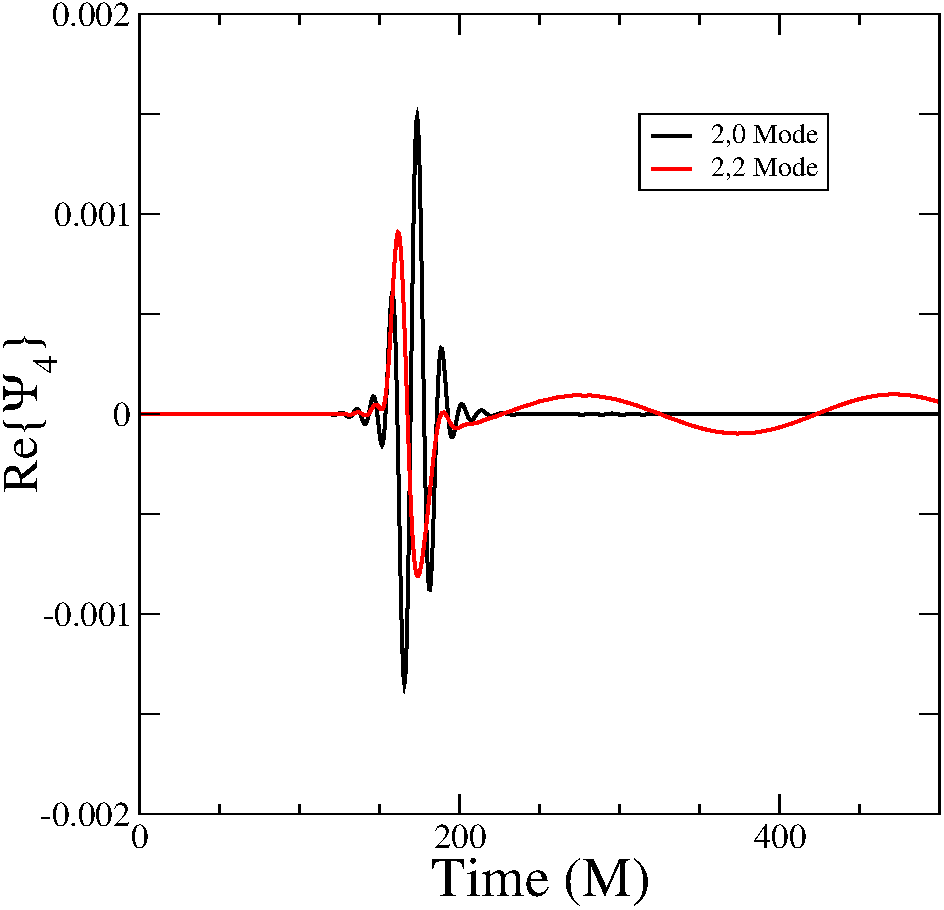
\includegraphics[scale=0.95]{chap5/Typical}
  \caption[A typical run illustrating junk radation.]{A typical run illustrating the spurious burst of junk radiation. At the very earliest times, no outgoing radiation has reached the extraction radius of $R=160M$. Then at $t\sim160M$, we see a burst of high-frequency, high-amplitude radiation. At later times, the $(2,0)$ mode dies out, and the $(2,2)$ mode settles into the usual inspiral radiation.}
  \label{fig:Typical}
\end{figure}


This junk radiation is undesirable in simulations for several
reasons. It adds to the computational cost of the simulation as the
junk radiation must leave the computational grid before any useful
physical information can be extracted. It can unrealistically shorten
the time until the black holes
merge~\citep{BodeEtAl:2008}. It also must be carefully considered when
comparing NR simulations with PN or EOB
calculations~\citep{Damour:2011fu}, or when creating PN/NR hybrid waveforms~\citep{MacDonald:2011ne}. It is therefore a useful endeavour to better
understand the junk radiation, how important it is, and how to reduce
it.

Junk radiation is thought to be caused by assumptions made during the
initial data construction, which are not compatible with binary black holes in perfect equilibrium. Specifically,
 black holes are generally treated in the
initial data as independent and non-interacting, while in reality
there should be some non-trivial tidal interactions between them which go unmodelled
(see~\cite{Chu:2014,JohnsonMcDaniel:2009dq} for examples of including tidal interactions). If
we consider a sequence of initial data sets where the initial
separation between the holes is decreasing, we would expect that these tidal interactions become more important as the initial separation
decreases. Similarly, to fully model binary black holes at a late stage of the inspiral,
there should already be some outgoing gravitational radiation already present in the initial data from its past history.
However, this is generally not explicitly modelled in current initial data codes (see~\big[\cite{JohnsonMcDaniel:2009dq,Kelly:2009js}\big] for efforts to model it).
Moreover, the black holes in the initial data are often constructed
with techniques that are incompatible a single, equilibrium black  hole.  Specifically, often, conformal flatness is assumed. As detailed in section~\ref{subsec:IVP}, the construction of initial data has a
free choice for the conformal metric, $\tilde{g}_{ij}$, on the initial
hypersurface. A common choice is conformal flatness, i.e.,
$\tilde{g}_{ij}$ is equal to the flat Euclidean metric, $f_{ij}$. Since every
spherically symmetric space is conformally flat, this is fine
for one Schwarzchild black hole. However,  a
binary system of compact objects is not conformally flat at second PN
order~\citep{Rieth:1997}. Moreover, the Kerr space-time does not admit a
conformally flat slicing that continuously approach Schwarzschild
coordinates as the spin goes to zero~\citep{GaratPrice:2000}. 
The former effect should decrease in importance with increasing separation of the binary.  The latter is caused by a deficiency of conformally flat slicing that is present even for single spinning black holes, and so we expect its importance
to be approximately independent of binary separation.

Superposed Kerr-Schild (SKS)~\citep{Matzner1999,Marronetti-Matzner:2000,Pfeiffer2002a,Lovelace2008} (conformally curved) initial data is now a common alternative to conformally flat initial data for binary black hole simulations.
The conformal metric is written as
\begin{equation}
\tilde{g}_{ij}=f_{ij}+e^{-(r_A/w)^2}\left(g_{ij}^A-f_{ij}\right)+e^{-(r_B/w)^2}\left(g_{ij}^B-f_{ij}\right),
\end{equation}
where $r^{A,B}$ are the distances
from black holes $A$ and $B$, and $g_{ij}^{A,B}$ is the Kerr-Schild metric boosted in
the direction of the black hole's motion. This has the effect that the
metric looks like Kerr-Schild near the black holes, and looks flat
far away. The Gaussian scalings help improve the
convergence of the initial data. SKS initial data is now the standard choice for all BBH simulations with spin done by the SXS collaboration, and was used in the creation of large waveform catalogs~\citep{Mroue:2013PRL,Chu:2015kft}. It has also been used in simulating black holes with nearly extremal spins~\citep{Lovelace:2011nu,Scheel2014,Lovelace:2014twa}. A similar approach has also been used for spinning black holes in BH-NS binaries(~\cite{FoucartEtAl:2008}, cf. Chap.~\ref{chap:bhns}). In contrast, CF initial data is used for non-spinning and low-spin ($\chi<0.5$) BBH simulations~\citep{Boyle2007,Buchman:2012dw,Chu:2015kft}.

\cite{Lovelace2009} investigated the effects on junk radiation of using SKS initial data for equal mass, non-spinning black
holes. It was found that in general, the
conformally curved initial data can decrease the amplitude of the junk
radiation by a factor of $\sim 2$.
Superposed Kerr-Schild initial data is built around the
  Kerr-Schild metric, which exactly represents single spinning black holes.
 Therefore, one would expect that the advantages of superposed Kerr-Schild become particularly apparent for spinning black holes.

In this paper we investigate the parameter space dependence of junk
radiation. We measure its dependence on the spin of the black holes and on their initial
separation, for low eccentricity, equal-mass,
spin-aligned binaries. We also perform a comparison between conformally
flat (CF) initial data and superposed Kerr-Schild (SKS) initial data. To
quantify the amount of junk radiation we will use three
diagnostics - the amount of energy present in the junk radiation, and
the size of the transient effects of mass increase and spin decrease
due to the junk radiation.

This chapter is organized as follows: 
  Section~\ref{sec:NumericalMethods} presents the numerical methods,
  and Section~\ref{sec:Methodology} describes how we quantify junk
  radiation and other initial transients in the BBH initial data sets.
  We present our results in Sec.~\ref{sec:Results} and close with a discussion in Sec.~\ref{sec:JRDiscussion}.

\section{Numerical Methods}
\label{sec:NumericalMethods}

\subsection{The Initial Value Problem}
\label{subsec:IVP}
Employing the usual 3+1 decomposition~\citep{ADM,york79}, space-time is foliated by a family
of spacelike hypersurfaces $\Sigma_t$. Each hypersurface has a
future-pointing unit normal $n^{\mu}$, induced metric $g_{ij}$, and
extrinsic curvature
$K_{\mu\nu}=-\frac{1}{2}\mathcal{L}_{n}g_{\mu\nu}$. The metric is
written as 
\begin{equation}
g_{\mu\nu}=-\alpha^2dt^2+g_{ij}\left(dx^i+\beta^idt\right)\left(dx^j+\beta^jdt\right),
\end{equation}
where $\alpha$ and $\beta^i$ are the lapse function and the shift vector
respectively. The lapse measures the proper time between neighbouring
hypersurfaces, and the shift vector determines how coordinate labels
move between neighbouring hypersurfaces.  On the initial
hypersurface $\Sigma_0$, spatial metric and extrinsic curvature must satisfy the vacuum
constraint equations
\begin{eqnarray}
R+K^2-K_{ij}K^{ij}&=&0, \\
\nabla_j\left(K^{ij}-g^{ij}K\right)&=&0.
\end{eqnarray}
% They are then evolved in time by the vacuum evolution equations
% \begin{eqnarray}
% \partial_tg_{ij}&=& blahblah \\
% \partial_tK_{ij}&=& blahblah 
% \end{eqnarray}
To solve the constraint equations one writes~\citep{Lichnerowicz44}
the metric in terms of a conformal metric $\tilde{g}_{ij}$ and a
conformal factor $\Psi$:
\begin{equation}
g_{ij}=\Psi^4\tilde{g}_{ij}.
\end{equation}
We also split the extrinsic curvature into trace and trace-free parts
\begin{equation}
K^{ij}=A^{ij}+\frac{1}{3}g^{ij}K,
\end{equation}
and employ the extended conformal thin sandwich formalism~\citep{York1999,Pfeiffer2003b} to further
decompose $A^{ij}$.  One must then choose
$\left(\tilde{g}_{ij},\partial_{t}\tilde{g}_{ij},K,\partial_{t}K\right)$
as the free data. Compared to the extrinsic curvature decomposition~\citep{Murchadha-York:1974b}, the conformal thin sandwich formalism allows for 
physically motivated choices to a larger number of the free data.  Elliptic equations
with appropriate boundary conditions are then solved for $\Psi$,
$\alpha\Psi$, and $\beta^i$, and the physical data is
re-assembled. $\partial_t\tilde{g}_{ij} = \partial_tK = 0$ is chosen
so that system is initially stationary in the co-rotating
frame.  This then leaves $\tilde{g}_{ij}$ and $K$ as the free data to
choose.  

The two types of initial data we compare are described in detail in~\cite{Lovelace2008}: conformally flat, quasi-equilibrium initial
data employs conformal flatness, $\tilde{g}_{ij}=f_{ij}$, maximal
slicing, $K=0$, and inner
boundary conditions that enforce that the black holes are
instantaneously in
equilibrium~\citep{Caudill-etal:2006,Cook2004,Cook2002}.  Superposed
Kerr-Schild initial data, first used
in~\citep{Marronetti-Matzner:2000,Matzner1999}\big], takes the spatial
metric and extrinsic curvature as superposition of elements of
Kerr-Schild metrics (one for each black hole).  As explained in~\cite{Lovelace2008}, we introduce Gaussian attenuation functions
to ensure regularity at spatial infinity. The details on the inner
boundary conditions used can be found in~\cite{Lovelace2008}.


\subsection{Code}
\label{sec:Code}

The initial data is solved using the spectral solver {\tt Spells}~\citep{Pfeiffer2003} of the Spectral 
 Einstein Code {\tt SpEC}\footnote{\url{www.black-holes.org}}. This is a
multi-domain elliptic PDE solver that uses pseudo-spectral methods,
whereby quantities of interest are expressed as a linear summation of
basis functions. This method gives exponential convergence (with the
number of basis functions) as long as the quantities of interest are
smooth. The black hole singularities are dealt with by excision from
the computational grid. We evolve the initial data with the dual frame method described in~\cite{Scheel2006}. The domain decomposition and position of the black
holes are fixed in a comoving frame, but the equations of motion are
solved in an inertial frame that is asymptotically Minkowski. The
frames are related by a rotation (due to orbital motion) and a
radial rescaling (due to inspiral motion).

Gravitational waves are extracted on outer spheres using the Newman-Penrose scalar $\Psi_4$. Given a spacelike
hypersurface with unit normal $n^{\mu}$ and a spatial unit vector in
the direction of wave propagation $r^{\mu}$, $\Psi_4$ is defined as 
\begin{equation}
\Psi_4 = -C_{\alpha\mu\beta\nu}l^{\mu}l^{\nu}m^{\alpha}\bar{m}^{\beta},
\end{equation}
where $C_{\alpha\mu\beta\nu}$ is the Weyl tensor,
$l^{\mu}=\left(n^{\mu}-r^{\mu}\right)/\sqrt{2}$ and $m^{\mu}$ is a
complex null vector satisfying $m^{\mu}\bar{m}_{\mu}=1$. We then expand
$\Psi_4$ in spin-weighted spherical harmonics
\begin{equation}
\Psi_4(t,r,\theta,\phi)=\sum_{l=2}^{l_{\rm max}}\sum_{|m|\leq~l}{\Psi_4^{lm}(t,r)_{-2}Y_{lm}(\theta,\phi)}
\end{equation}
The number of terms used in this expansion is generally $l_{\rm max}\leq 8$ in
our simulations. At large $r$, $\Psi_4$ is related to the
gravitational wave amplitude, $h$, by
\begin{equation}
\Psi_4=\frac{d^2}{dt^2}h_{+}-i\frac{d^2}{dt^2}h_{\times}.
\end{equation}


\subsection{Eccentricity Reduction}
Gravitational radiation tends to circularize in-spiralling compact
binaries~\citep{PetersMathews1963,Peters1964}. We reduce orbital
eccentricity with an iterative method similar to the one described in~\citep{Boyle2007,Chu2009}. One selects the initial orbital
frequency $\Omega_0$ from Kepler's third law or from a Post-Newtonian
calculation, while assuming that the initial radial velocity, $v_r$ is
zero. After the first simulation has run for a sufficient length, about two orbits, we fit the time derivative of
the orbital frequency, $\dot{\Omega}(t)$ as suggested
in~\cite{Buonanno:2010yk}, to the function
%We fit parameters $\{A_0, A_1, \tau, B, \phi, \omega, q\}$ with the function
\begin{equation}
\label{eq:eccfit}
\dot{\Omega}(t)=A_0\left(\tau-t\right)^{-11/8}+A_1\left(\tau-t\right)^{-13/8}
+B\cos\left(\varphi + \omega
  t+qt^2\right).
\end{equation}
Here $\{A_0,A_1,B,\varphi,\omega,q,\tau\}$ are the fitted parameters. The first two terms in Eq.~\ref{eq:eccfit} represent the
smooth inspiral motion of the black holes, with functional form motivated by PN calculations~\citep{Blanchet:2009rw}. The oscillatory term captures effects due to eccentricity. After the trajectories of an evolution have been analyzed via the fit in Eq.~\ref{eq:eccfit}, we update the parameters with
\begin{equation}
\delta\Omega_0=-\frac{B\omega\sin{\varphi}}{4\Omega_0^2},
\end{equation}
\begin{equation}
\delta v_r = \frac{B d_0\cos{\varphi}}{2\Omega_0},
\end{equation}
where $d_0$ is the binary separation. These updates are designed to circularize low eccentricity Newtonian binaries. The eccentricity of the binary is estimated as~\citep{Buonanno:2010yk},
\begin{equation}
e = \frac{|B|}{2\Omega_0^2}.
\end{equation}
 This
process is continued iteratively, typically another one or two times,
until the eccentricity is reduced to $e\lesssim 0.002$. The effect of
eccentricity on junk radiation is discussed in section~\ref{subsec:ErrorEstimation}.

\subsection{Simulations}

We run BBH evolutions using both conformally flat and SKS initial
data.  We consider five different initial separations for CF data,
$D/M=\{12,15,20,25,30\}$, and $D/M=\{12,15,20\}$ for SKS data, where $M$ is the total mass of the binary.
holes. At each separation we consider  six different spins,
$\chi=\{0,0.1,0.2,0.3,0.4,0.5\}$. In each case the black holes are of
equal mass, equal spin, and the spin is aligned with the orbital
angular momentum, i.e., in the the $+\hat{z}$ direction. To test the
convergence of our measurements, each run is done at four
resolutions, which we will refer to as {\tt N0} (lowest resolution) to
{\tt N3}
(highest resolution). Each evolution is
run to about $t\sim1000M$, which is long enough to accurately measure the
eccentricity, and make sure that it is sufficiently low for our purposes, i.e.,
$e\lesssim 0.002$.

%%%%%%%%%%%%%%%%%%%%%%%%%%%%%%%%%%%%%%%%%%%%%%%%%%%%%%%%%%%%%%%%
\section{Methodology}
\label{sec:Methodology}
%%%%%%%%%%%%%%%%%%%%%%%%%%%%%%%%%%%%%%%%%%%%%%%%%%%%%%%%%%%%%%%%

We employ three diagnostics to measure the initial relaxation of
the initial data: the outgoing pulse of radiation (junk radiation),
the change in black hole mass during relaxation, and the change in
black hole spin during relaxation.



\subsection{Pulse in the Gravitational Waveform}

In this section we discuss our methods of
quantifying the amount of junk radiation present in a given
simulation. It is not immediately obvious what the best way to do this
is.~\cite{Lovelace2009} considered the
maximum value of the Newman-Penrose waveform,
$\max\{R|\Psi_4^{lm}|\}$, where $R$ is the extraction radius of the gravitational waves.  The
  $(l,m)=(2,2)$ and $(2,0)$ modes were found to dominate. We find,
  however, that this method has some inadequacies. This is illustrated
  by comparing $R|\Psi_4^{lm}|(t_R)$, where $t_R$ is the retarded time,
  $t_R=t-R$, in two different simulations. These use CF data, with the parameters $\{D=15M$, $\chi=0.2\}$; one is at our
  typical highest resolution {\tt N3}, and another at an even higher
  resolution, {\tt N7}. In terms of the total number of basis
    functions $X$, $X^{1/3}\sim58$ for {\tt N3} and $X^{1/3}\sim78$ for
    {\tt N7}. The $(2,0)$ and $(2,2)$ modes are shown in the top panel of
  Fig.~\ref{fig:HighResComparison}. It is clear that the $(2,0)$ mode
  is significantly different between {\tt  N3} and {\tt N7}, in both the
  largest peak and in the subsequent smaller peaks, and that these
  differences are not well captured simply by using
  $\max\{R|\Psi_4|\}$. In Fig.~\ref{fig:HighResComparison} we also
  show these quantties for an SKS run with the same parameters. Because
  the waveform is significantly different from the CF waveform in both the
  number of peaks and their relative heights, it is clear that
  $\max\{R|\Psi_4^{lm}|\}$ does not encapsulate this waveform very well.

%\red{[Shorten this paragraph, combine with above.  The purpose of this paragraph is to explain why we do not follow Lovelace 2009, and this can be done with fewer words.  Although it would be handy to have a SKS Psi4 waveform, to further illustrate the problems. 
%]}
%We find, however, that this method presents several problems.  We compare two runs with evolution parameters $D=15M$ and
%$\chi=0.2$ and conformally flat initial data. One run
%is at our normal highest resolution, Lev3, and another is a very high
%resolution at Lev7. In terms of total number of basis functions, N, these
%resolutions are $N^{1/3}=57.93$ and $N^{1/3}=78.04$, respectively. In
%Fig.~\ref{fig:HighResComparison} we show the junk radiation
%content of the $(2,0)$ and $(2,2)$ modes for both of these runs.\note{Somewhere in here discuss the SKS part of fig2} The
%$(3,2)$ mode also has a significant contribution, but it is omitted
%for clarity. Clearly $\max\{r|\Psi_4^{lm}|\}$ has a quite
%strong dependence on resolution, especially in the $(2,0)$ mode. However,
%another problem is quite evident. For the $(2,0)$ mode, the first peak
%is much higher at Lev7, but the second peak is close, and all
%subsequent peaks are significantly smaller. Thus, in using
%$\textnormal{max}\{r|\Psi_4^{l,m}|\}$, important features in the junk
 %radiation are lost. Thus we conclude
%that $\textnormal{max}\{r|\Psi_4^{l,m}|\}$ is not a suitable diagnostic 
%for the amount of junk radiation.

\begin{figure}
  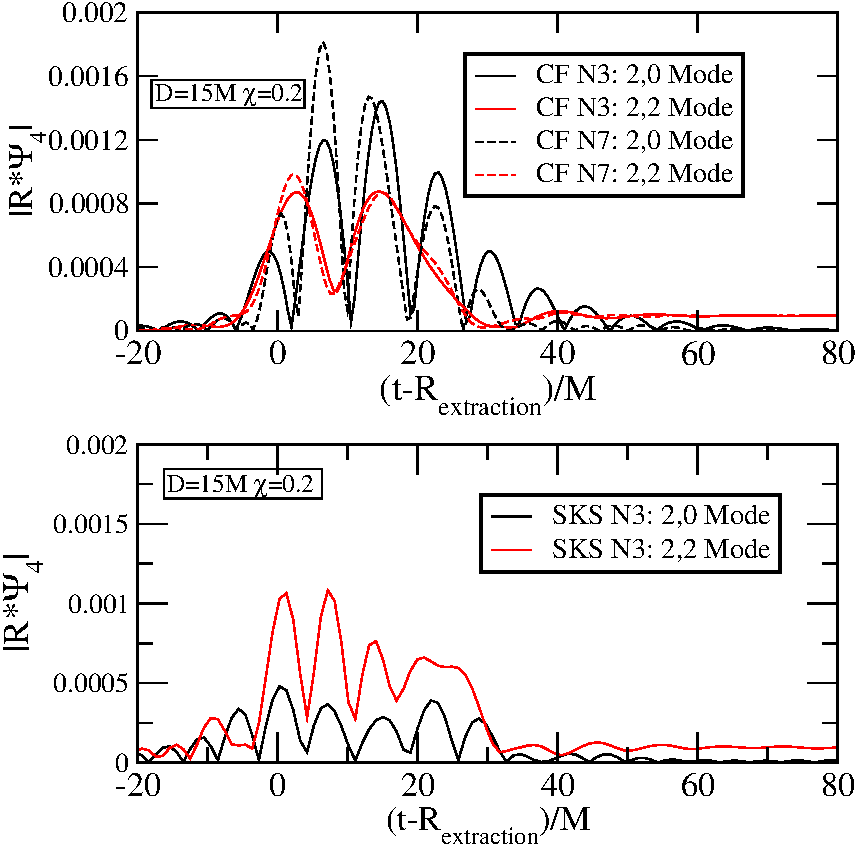
\includegraphics[scale=0.95]{chap5/HighResComparison}
  \caption[Junk radiation profiles for CF and SKS initial data.]{
%{\red{Consider moving fig forward a page}
{\it Top Panel:} Comparison of the junk radiation profiles for our usual
    highest resolution ({\tt N3}) and an additional run at a much higher
    resolution ({\tt N7}). We see, especially for the $(2,0)$ mode, that the
    maximum peak of the junk radiation is much higher for {\tt  N7}, but
    additional peaks are comparable or higher for {\tt N3}. \newline {\it
      Bottom Panel:} Junk radiation profile for an SKS run with the
    same parameters as in the top panel. The waveform is significantly
    different in structure from the CF waveform.
}
  \label{fig:HighResComparison}
\end{figure}

As a more robust quantity that incorporates the whole waveform, and is
less resolution dependent than $\max\{R|\Psi_4^{lm}|\}$, we consider the
total energy carried away from the system by gravitational waves. The
 gravitational wave energy flux is~\citep{Boyle:2008}
\begin{equation}
F(t) =\frac{1}{16\pi}\sum_{l,m}\dot{h}_{lm}^2(t),
\end{equation}
where
\begin{equation}
\dot{h}_{lm}(t)=\int_{t_0}^{t}{\Psi_4^{lm}(t')dt'} + H_{lm}.
\end{equation}
The $H_{lm}$ are integration constants.  To measure the
  initial pulse of radiation, we use $t_0=0$ and $H_{lm}=0$.  The energy flux, $F(t)$, is shown in
the red curves in Fig.~\ref{fig:FluxSample} for conformally flat initial data (top
panel) and SKS initial data (bottom panel).  The initial burst
  is apparent in these figures; at late times $t_R\gtrsim 40M$, $F(t)$
  approaches the nearly constant energy flux of the astrophysical
  inspiral.  We are now faced with two problems: We would like to
  isolate the energy carried in junk-radiation from the energy-flux
  astrophysical inspiral.  And, we would like to do so in a robust way, 
independent of arbitrary choices.  We
  proceed as follows:

  First, we assume that the astrophysical energy flux begins at a time
  $t_{22}$, i.e.
\begin{equation}
  F_{22}(t) = F_0\,\theta(t-t_{22}).
\end{equation}
Here, $F_0$ represents the value of $F(t)$ after the pulse of
junk-radiation and $\theta$ represents the step-function.
The choice of a constant value $F_0$ is reasonable since the
timescale on which $F_{22}$ changes significantly is much longer than
the junk radiation timescale.
We will
discuss our choice for $t_{22}$ shortly.  The energy in the
junk-radiation is now taken as
\begin{equation}\label{eq:EJ}
E_J=\int_0^{t_C}\big[(F(t)-F_{22}(t)\big]dt,
\end{equation}
where the cut-off time $t_C$ is chosen after the junk radiation has
decayed, i.e. $t_C-R\gtrsim 50M$.  In Fig.~\ref{fig:FluxSample} we
plot a representative example of the computation of $E_J$ for CF (top
panel) and SKS (bottom panel) data. The blue dashed curves represent
$F_{22}(t)$, while the shaded area represents $E_J$.
%The energy attributed to the junk
%radiation is thus the shaded area in Fig.~\ref{fig:FluxSample}.  
As
already apparent from Fig.~\ref{fig:FluxSample}, the precise value of
$t_C$ is not extremely important, because at late times $F(t)-F_{22}(t)\approx 0$.  

It remains to chose a prescription for the choice of $t_{22}$, the
time when we deem the astrophysical waveform to ``turn on''.
% In finding the total energy in junk radiation, however, it cannot
% be assumed that all the energy emitted up to $t=t_C$ is due to junk
% radiation. The astrophysical $2,2$ mode signal, $F_{22}(t)$, should
% still be present, with the junk radiation signal superimposed on
% it. The energy in junk radiation is thus written as
% \begin{equation}
% E_J=\int_0^{t_C}\left(F(t)-F_{22}(t)dt\right)
% \end{equation}
% This quantity is represented by the shaded area in
% figure~\ref{fig:FluxSample}. We choose a simple model for $F_{22}(t)$:
% $F_{22}$ turns on at some time $t_{22}$ and takes on the constant
% value of $F_0=F(t_C)$. That is,
% \begin{equation}
% F_{22}(t)=F_0\theta\left(t-t_{22}\right)
% \end{equation}
% This is represented by the blue curves in
% figure~\ref{fig:FluxSample}. 
%The choice of a constant value for the flux is reasonable since the
%timescale on which $F_{22}$ changes significantly is much longer than
%the junk radiation timescale. 
%There is no a priori way to precisely
%determine where $t_{22}$ should be. 
A simple method would be to choose
$t_{22}$ to correspond to $\max\{F(t)\}$. This seems reasonable for
the conformally flat curve in Fig.~\ref{fig:FluxSample}, but the
more wide double-peaked structure of the SKS curve shows that another
approach is needed. Instead we take $t_{22}$ to correspond to the flux
weighted centre of the junk radiation waveform. The first moment of
$F(t)-F_{22}(t)$, in other words. So,
\begin{equation}\label{eq:t22}
t_{22}=\frac{\int_0^{t_C}{t\left(F\left(t\right)-F_0\theta\left(t-t_{22}\right)\right)dt}}{\int_0^{t_C}{\left(F\left(t\right)-F_0\theta\left(t-t_{22}\right)\right)dt}}.
\end{equation}
This equation is solved iteratively for $t_{22}$.

\begin{figure}
 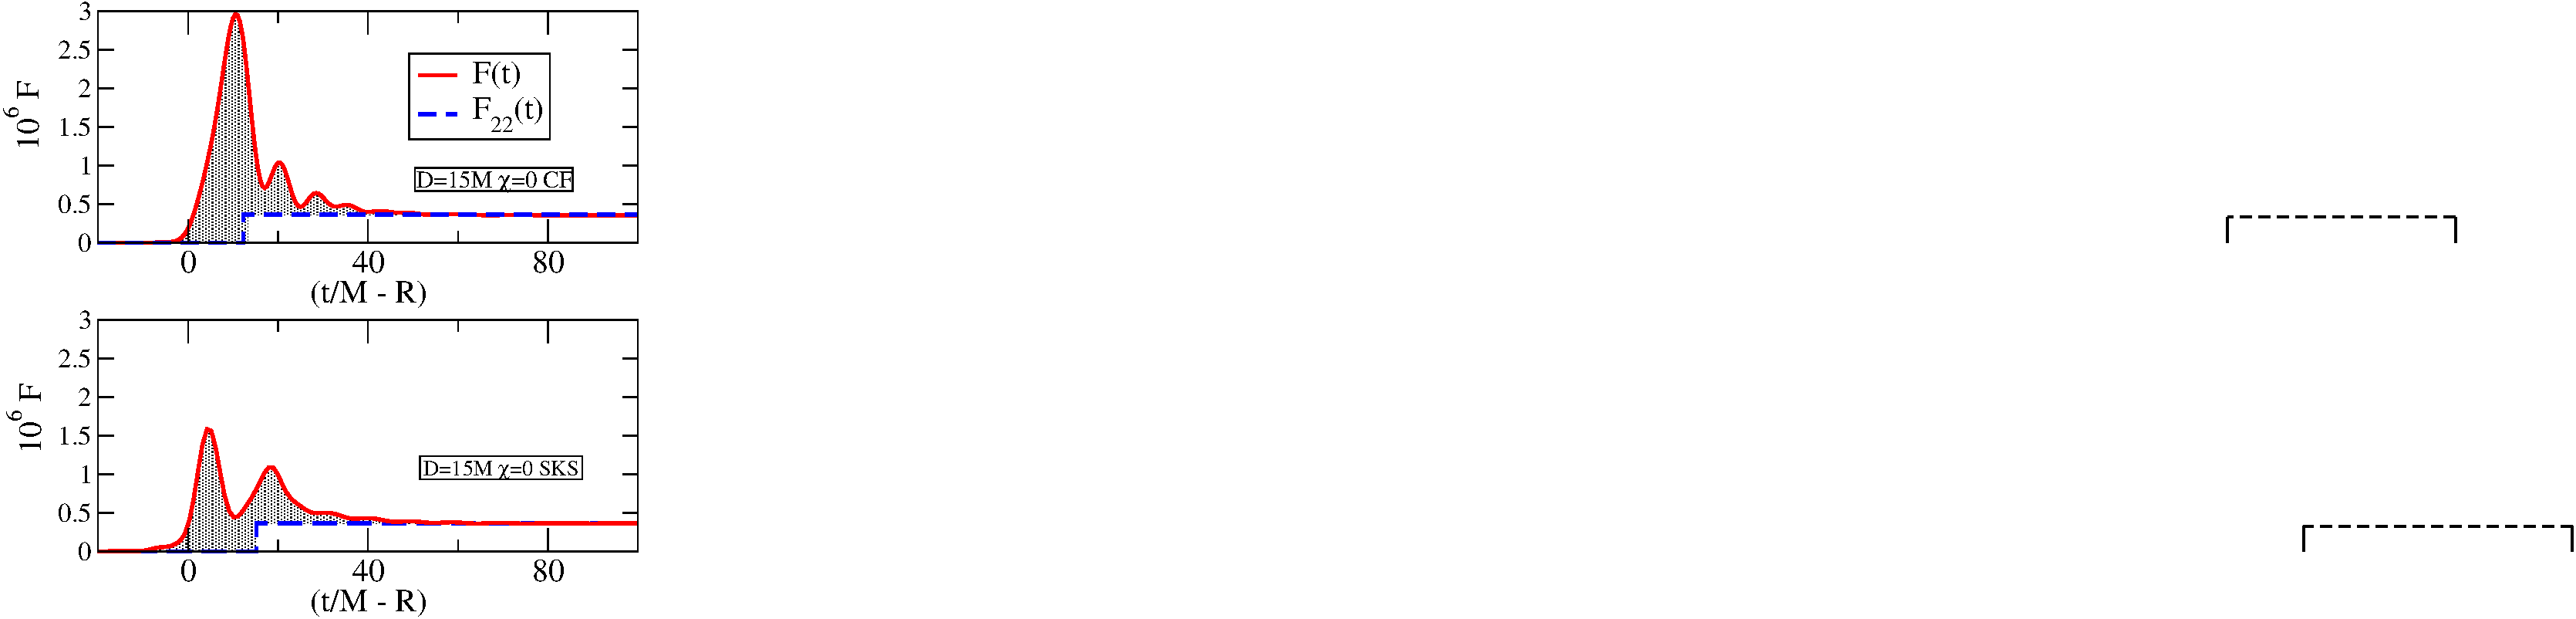
\includegraphics[scale=0.95]{chap5/FluxSample}
  \caption[The flux, $F(t)$, and the computation of $E_J$ for CF and
  SKS intitial data.]{
%{\red{Consider moving fig forward 1-2 pages.} \red{Show same runs as in Fig 4.2}
The flux $F(t)$ is plotted for two different runs, both
    with parameters $D=15M$ and $\chi=0$. Conformally flat initial
    data is in the top panel and SKS initial data is in the bottom
    panel. The solid red curve represents the total flux, $F(t)$. The
    dashed blue curve represents $F_{22}(t)$, the astrophysical flux
    that we subtract from $F(t)$. The shaded area between the two
    curves is the energy in junk radiation, $E_J$.
}
  \label{fig:FluxSample}
\end{figure}

\subsection{Uncertainty in $E_J$}
\label{subsec:ErrorEstimation}

%\subsubsection{Resolution of the Waveform}

Several effects may influence the quantity $E_J$ computed by
  Eqs.~(\ref{eq:EJ}) and~(\ref{eq:t22}).  {\it Numerical truncation
    error} can be estimated by performing the simulations with
  different numerical resolution.  Our simulations show that in general,
  $E_J$ increases with resolution. This is because junk radiation is
a short wavelength feature, so greater resolution allows for more of
the features present to be captured.  To estimate the
uncertainty in $E_J$, we compare our $\{D=15M$,
$\chi=0.2\}$ runs at {\tt N3} and {\tt N7}, as discussed earlier. We find that
at {\tt N7}, $E_J$ is about $13\%$ greater than at {\tt N3}. Since we don't
have such high resolutions runs available for each of our cases, we
assume that we can use this same $13\%$ difference for each of our
runs. We are also assuming that at {\tt N7} the junk
radiation is nearly fully resolved, so that this difference is a good
indication of the true value. Finally, we use this same uncertainty of
$13\%$ for the SKS runs as well - while the technology is different
for the SKS runs, it should still be a reasonably good estimate of the numerical truncation error in them.

%\subsubsection{Choice of $t_C$}

A second uncertainty arises through the {\it choice of~$t_C$}.
This number is chosen manually for
each run, introducing a
  subjective element into the analysis. Examining the flux curves in
Fig.~\ref{fig:FluxSample}, for example, $t_C$ could conceivably be
chosen differently by $\sim 10 M$ and still be a
reasonable choice. {Our definition Eq.~(\ref{eq:EJ}) was meant
to be robust to small changes in $t_C$.  For $E_J$ to be a robust measurement, it should
therefore not change significantly in response to changes $\delta t_C$
that are of that order. Indeed, this is enforced by our definition of
$E_J$, which subtracts out the additional flux in the astrophysical
$(2,2)$ mode.}  To verify this assertion, we compute $E_J$ with $t_C$ in Eq.~(\ref{eq:EJ}) replaced by $t_C+\delta t_C$.  Figure~\ref{fig:EvsDtC} shows that indeed $E_J$ is almost independent of $\delta t_C$.  
%The uncertainty introduced by $t_C$ is about $1\%$. 
In Fig.~\ref{fig:EvsDtC}, $E_J$ is plotted against $t_C$
in the representative $\{D=15M, \chi=0\}$ case.
For each run we define a fractional
error parameter due to the choice of $t_C$, where we average the
differences for $\delta t_C = -10M$ and $\delta t_C = 10M$:
\begin{equation}
\frac{\Delta E}{E} = \frac{|E_J(t_C+10M) - E_J(t_C)| + |E_J(t_C) - E_J(t_C -
  10M)|}{2E_J(t_C)}
\end{equation}
This uncertainty ranges from $\sim 0.25\%$ to $\sim 3.75\%$ throughout
all of our simulations.

\begin{figure}
 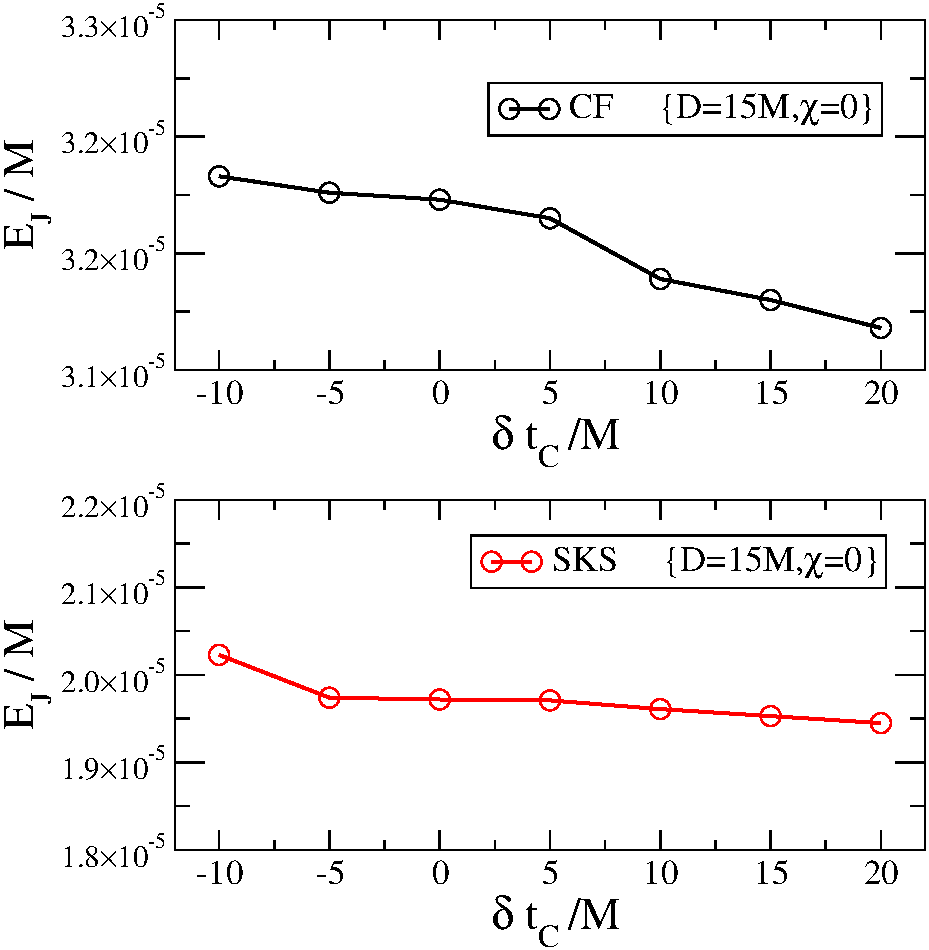
\includegraphics[width=0.95\columnwidth]{chap5/EvsDtj}
  \caption[$E_J$ as a function of $\delta t_C$.]{$E_J$ is plotted against $\delta t_C$, representing changes
    to the selected value of $t_C$ for runs where $D=15M$,
    $\chi=0$. The results for conformally flat initial data are shown
    in the top panel, and SKS initial data in the bottom
    panel. Typical changes in $E_J$ are on the order of a few
    percent.}
 \label{fig:EvsDtC}
\end{figure}


A third error in $E_J$ arises through {\it the finite radius
    of gravitational wave extraction}.  In this study, gravitational waves are extracted at radii $R_{\rm ex}\sim 300-400M$.  Gravitational waves extracted at finite radii are subject to near-field effects which may cause the extracted
waveforms to differ from the one that would be observed at
infinity.  
To estimate the error in $E_J$ due to the finite extraction radius, we
use the following procedure. For each of our simulations, we compute $E_J$ at
several extraction radii, and examine $E_J$ as a function of
$1/R_{ex}$. We then extrapolate
\begin{equation}
E_{\infty} = \lim_{1/R_{ex}\rightarrow 0}E_J(1/R_{\rm ex})
\end{equation}
using a linear fit in $1/R_{\rm ex}$ to estimate the behaviour of $E_J$ at infinity. We
then take the fractional difference
\begin{equation}
\frac{\Delta E}{E} = \frac{E_{\infty}-E_J}{E_J}
\end{equation}
as our error estimate. This parameter is on the order of $10\%$ for
most of our runs. Note, however, that we still use $E_J$ and not $E_{\infty}$ as
our measure of energy in the pulse. In Fig.~\ref{fig:EvsRextr} we illustrate an
example of this procedure, plotting $E_J$ vs. $1/R_{ex}$ for one case,
$\{D=15M, \chi=0\}$, for both CF and SKS data.

\begin{figure}
  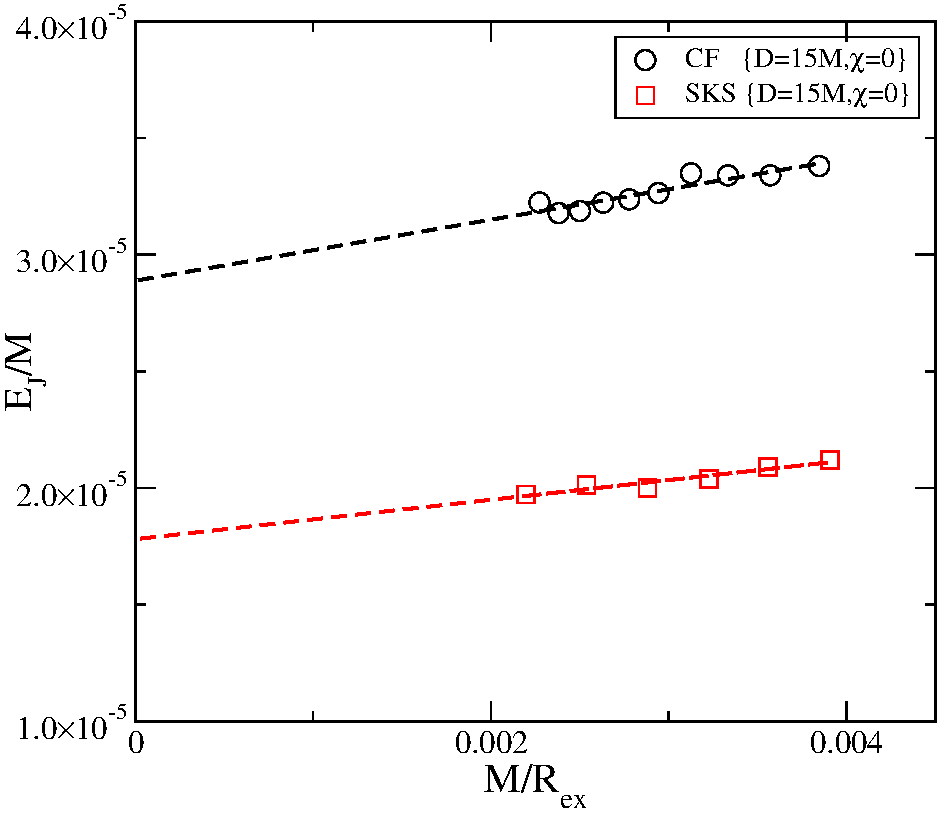
\includegraphics[scale=0.95]{chap5/EvsRextr}
  \caption[$E_J$ as a function of $1_R/{\rm ex}$.]{$E_J$ as a function of $1/R_{ex}$, where $R_{ex}$ is the
    extraction radius. This is for the case where $\{D=15M,\chi=0\}$,
    with CF data in black and SKS data in red. The dashed lines
    represent the best linear fit. The extrapolation
    to $1/R_{ex}\rightarrow 0$ allows us to estimate the error on
    $E_J$ due to finite extraction radius effects. }

  \label{fig:EvsRextr}
\end{figure}

A final factor that could influence the estimated $E_J$ is the
{\it eccentricity of the orbit of the black holes}. Previously we argued
that astrophysically realistic binaries have
low eccentricity. Because our NR simulations cannot be run at precisely $e=0$, we now consider how a small residual eccentricity affects the junk radiation, specifically the computed $E_J$. We examine the case $\{D=25M,\chi=0.1\}$
for CF data, as this particular case encountered a fairly large range of
eccentricities in the eccentricity reduction process;
$e\sim\{0.03,0.008,0.0006\}$. The measured $E_J$ for these three cases
is $10^6E_J=\{7.053\pm0.38\%, 7.204\pm0.53\%, 7.174\pm0.58\%\}$. Here,
the quoted uncertainty is purely due to the choice of $t_C$. The
differences between the first two eccentricities is $2.10\%$ and it is
$0.42\%$ for the last two. Because the latter difference is less than
the uncertainty due to the choice of $t_C$, the two runs are
effectively indistinguishable, and we conclude that we can safely
ignore the effects of residual eccentricity once we have $e\lesssim
0.008$. However, to be ``safe'', we have generally reduced the
eccentricity of all of our runs to $e\lesssim 0.002$.

%\harald{A final factor influencing the estimated $E_J$ is the
%{\em eccentricity of the orbit of the black holes}. }
%\subsubsection{Effect of Eccentricity}
%\label{subsec:EccentricityEffect}
%\red{[As discussed: Remove Fig.~\ref{fig:EccComparison}, state here in main-text $E_J$ for the different eccentricities, conclude that the effect of eccentricity is below xxx.  Also shorten text, by removing unneeded words and information] }
%Previously, we argued that it is important for astrophysically
%realistic binaries to have low eccentricity. We now examine how
%eccentricity actually affects the junk radiation. In
%figure~\ref{fig:EccComparison}, we have plotted the leading order (2,0) mode
%of the junk radiation for eccentricities of $e\approx
%\{0.03,0.008,0.0006\}$. This was done for runs where $D=25M$,
%$\chi=0.1$, and at medium resolution, i.e. Lev2. This was chosen as it
%happened to give us the largest range of eccentricities available, and
%often the highest resolution Lev3 runs at higher eccentricity were
%terminated earlier. We find that the junk radiation amplitude is
%nearly independent of the eccentricity. Figure ~\ref{fig:EccComparison} shows
%that there is some visible difference between
  %$e\approx 0.03$ and $e\approx 0.008$, but nearly no difference
  %between $e\approx 0.008$ and $e\approx 0.0006$.  The impact of eccentricity
%on the junk-radiation is even smaller for the $(2,2)$
  %mode. Figure~\ref{fig:EccComparison} essentially shows that we can
  %safely ignore the effects of residual eccentricity once we have $e
  %\lesssim 0.008$. However, to be ``safe'', we have generally reduced
  %the eccentricity of all of our runs to $e\lesssim 0.002$.
%\begin{figure}
%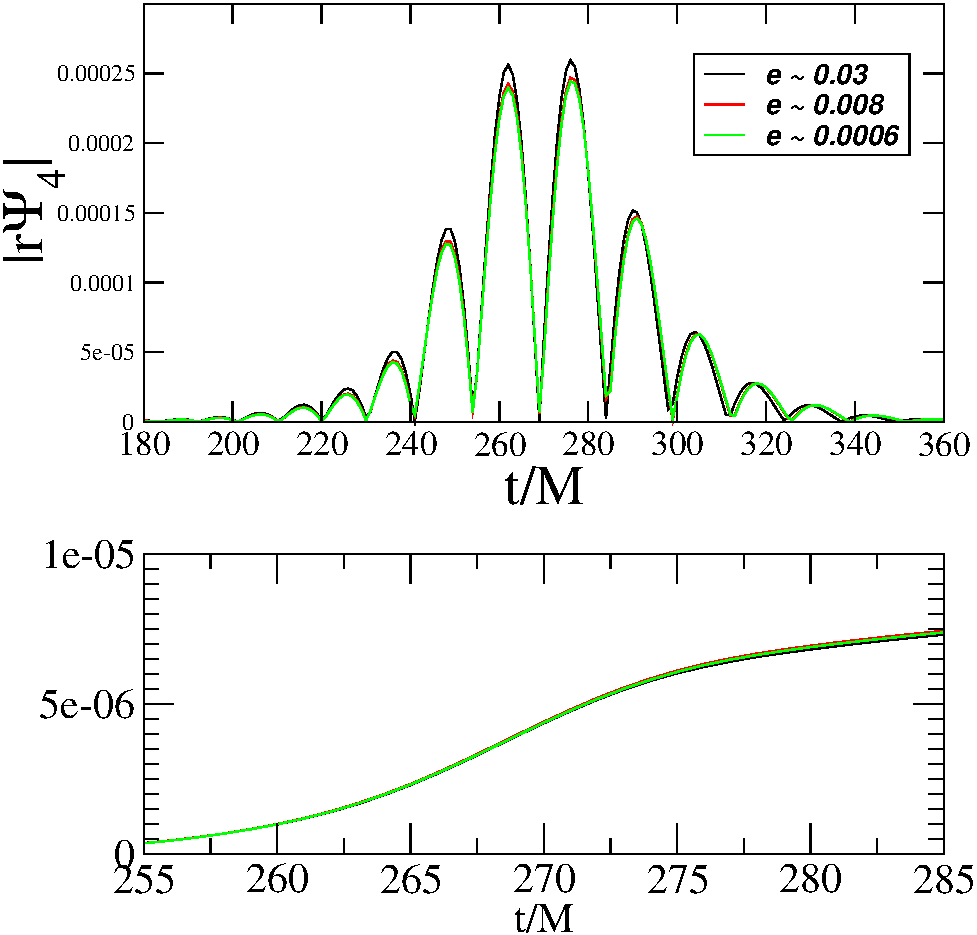
\includegraphics[scale=0.5]{EccComparison}
 % \caption{\note{Kill this plot, and add words describing it to the text}\note{Define what is plotted.  If this is the integral of
%      $\dot h_{20}^2$, then wouldn't it be more suitable to plot
 %     $E(t)$ directly at different resolutions?  Include legend} A
   % comparison of the $2,0$ mode of junk radiation at three different
   % eccentricities. At the two lowest eccentricities, the junk
   % radiation profiles are essentially the same, telling us that we
   % can effectively ignore eccentricities under $e \sim
   % 0.008$}
 % \label{fig:EccComparison}
%\end{figure}

\subsection{Transient Behaviour in Black Hole Quantities}

\subsubsection{Mass Increase}
In addition to the energy carried away in junk radiation, we utilize two further
diagnostics of transients arising from imperfect initial data.
The first diagnostic comes from the irreducible
mass of the black hole, $M_{\rm irr} = \sqrt{A/16\pi}$, where $A$
is the area of the black hole's apparent horizon. In the first few $M$ during the evolution, the apparent horizon mass
$M_{\rm irr}(t)$ increases by a small amount, before settling down to
an approximately constant value. This effect is visible in Fig.~\ref{fig:MassIncreaseCFSKS} for $0\le~t/M\le10$.
We characterize the increase in mass due to initial transients by 
\begin{equation}
\delta M(t)=\frac{M_{\rm irr}(t)}{M_{\rm irr}(0)}-1
\end{equation}
and we define the equilibrium parameter $\delta M = \delta M(t_{\rm eq})$.
Here $t_{\rm eq}$ is a time where the mass-increase is complete has and
levelled off; typically $\sim20M$. 

For SKS initial data the behaviour of $M_{\rm irr}(t)$ is more
  complex.  Within the first few $M$, $M_{\rm irr}(t)$ shows a rapid
  increase, presumably due to relaxation of the geometry
  in the immediate vicinity of the black holes.  The trend here is
  similar to the CF initial data, in that larger spins result in a
  larger increase of $M_{\rm irr}(t)$, albeit the magnitude of the
  increase is about a factor of 50 smaller for SKS initial data.
  Subsequently, starting at $t\sim 40M$, the SKS simulations show a second
  set of features, oscillations with amplitude $\sim 2\times 10^{-5}$ lasting about
  $60M$.  The features of these oscillations are similar to each other
  even for runs with different spin black hole spin $\chi$.  Therefore, it is
  likely that these oscillations are caused by features in the initial
  data set {\it away} from the black holes.

\begin{figure}[!htb]
 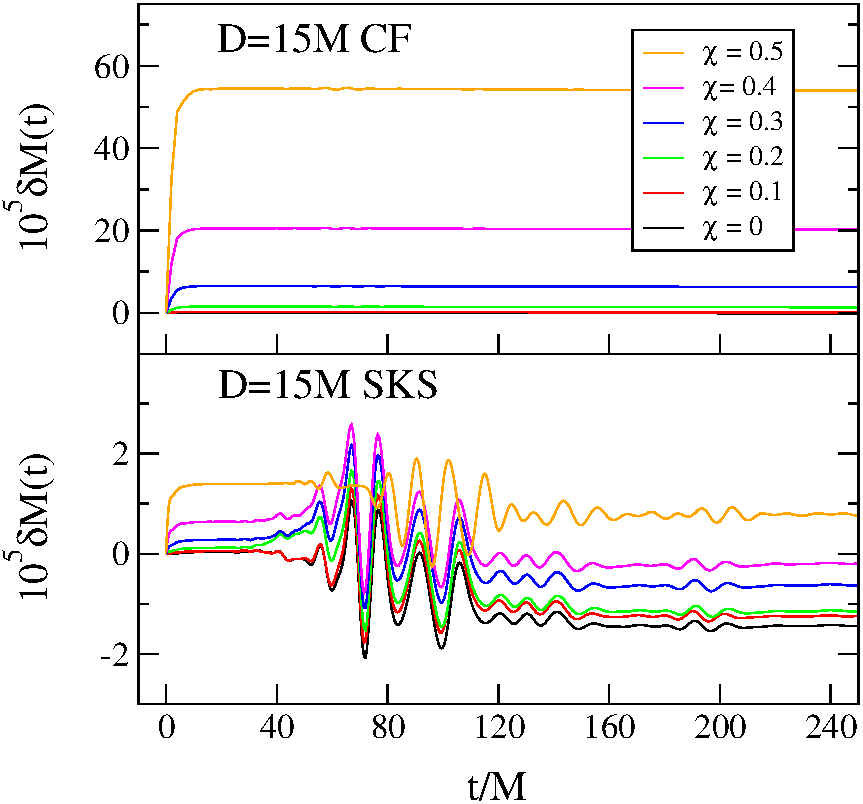
\includegraphics[width=0.95\columnwidth]{chap5/MassIncreaseCFSKS}
  \caption[Normalized change in irreducible mass curves for CF and SKS data.]{Normalized change in irreducible mass curves for CF data (top panel)
    and SKS data (bottom panel) for all of the different spins in the
    covered parameter space and $D=15M$ remaining constant. }
  \label{fig:MassIncreaseCFSKS}
\end{figure}

There is a clear qualitative difference between the CF and SKS
curves. The CF data forms an increasing sequence of
$\delta_M$ with $\chi$, and $\delta_M$ is clearly well-defined in each
case. However, the SKS data exhibits oscillatory behavior that is
relatively spin-independent, and there is not a clear way to robustly
define $\delta_M$. To further underscore the difficulties of the SKS
data, figures~\ref{fig:CFMConvergence1} and~\ref{fig:SKSMConvergence1}
show convergence tests for one of the mass curves shown in
fig.~\ref{fig:MassIncreaseCFSKS}, $\{D=15M,\chi=0.3\}$. The top panels
of Figs.~\ref{fig:CFMConvergence1} and~\ref{fig:SKSMConvergence1} show
$M_{\rm irr}(t)$ of one of the black holes computed at different
numerical resolutions, and the bottom panels show differences in
$M_{\rm irr}(t)$ computed at neighboring resolutions. Note that our
parameter space studies presented in Sec.~\ref{sec:Results} were
usually performed on resolution {\tt N3}; we have run {\tt N4-N6} for
select cases to test convergence. The CF initial data shows rapid
convergence and the features in the upper panel of
Fig.~\ref{fig:CFMConvergence1} are well resolved. For the SKS data
shown in Fig.~\ref{fig:SKSMConvergence1} we do not find convergence -
the differences between resolutions do not strictly decrease with
increasing resolution, and these differences are of similar order to
the features that we are trying to quantify. Our conclusion is
therefore that the magnitude of the change $M_{\rm irr}(t)$ 
%is much
%smaller for SKS initial data than for CF initial data ($\sim 10^{-5}$
%vs. $\sim 5\times10^{-4}$), however, the changes in $M_{\rm irr}(t)$
for SKS initial data approaches our numerical truncation error, and are
furthermore ambiguous due to the extra oscillatory features present in
Fig.~\ref{fig:MassIncreaseCFSKS}. In the parameter space survey of junk radiation in Sec.~\ref{sec:Results} below, we will not attempt to
quantify them in detail, beyond giver upper bounds on $\delta_M$ for
the SKS data.

\begin{figure}
 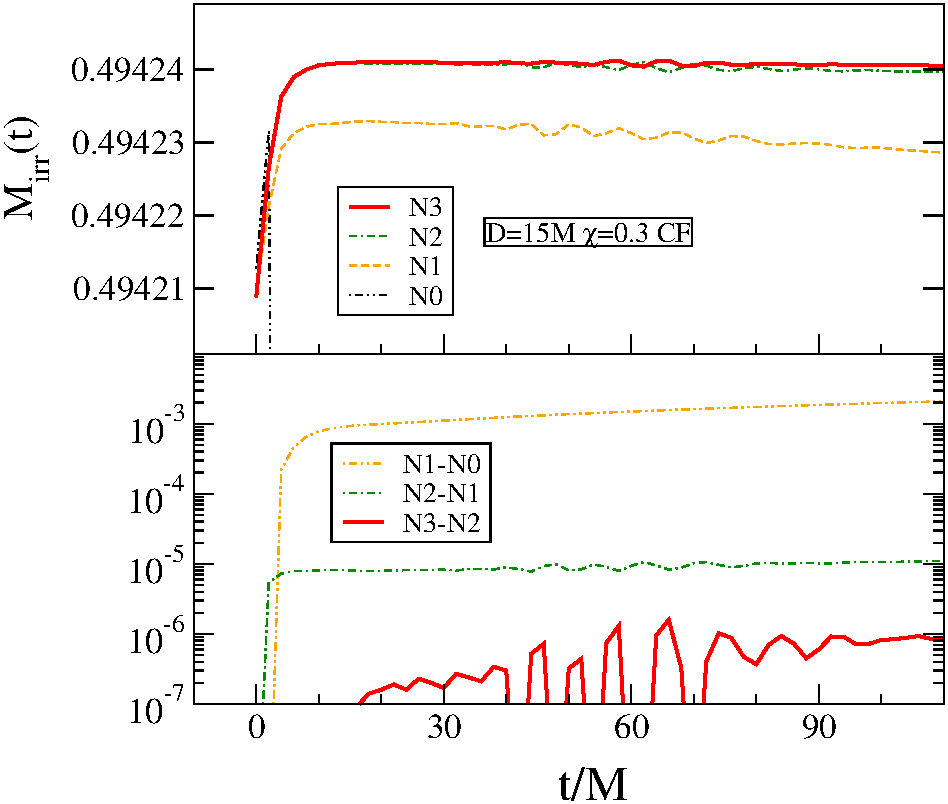
\includegraphics[scale=0.95]{chap5/CFMConvergence1}
  \caption[Convergence of $M_{\rm irr})(t)$ for CF initial
  data.]{Convergence test of $M_{\rm irr}(t)$ for CF initial data in the
  case $\{D=15M,\chi=0.3\}$. The top panel shows $M_{\rm irr}(t)$ at
  different resolutions, and the bottom panel shows the difference
  between consecutive resolutions.}
  \label{fig:CFMConvergence1}
\end{figure}

\begin{figure}[!htbp]
 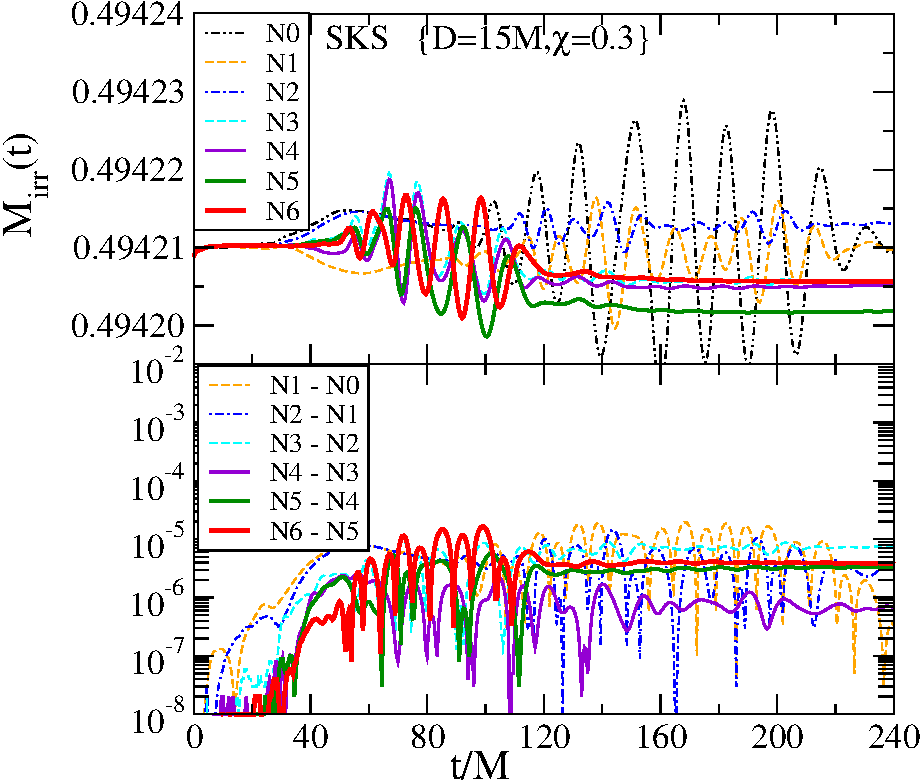
\includegraphics[scale=0.95]{chap5/SKSMConvergence1}
  \caption[Convergence of $M_{\rm irr})(t)$ for SKS initial
  data.]{Convergence test of $M_{\rm irr}(t)$ for SKS initial data in the
  case $\{D=15M$, $\chi=0.3\}$. The top panel shows $M_{\rm irr}(t)$ at
  different resolutions, and the bottom panel shows the difference
  between consecutive resolutions.}

  \label{fig:SKSMConvergence1}
\end{figure}

\subsubsection{Spin Decrease}

Our third and final quantification of junk radiation comes from the
black hole's spin $S(t)$. At early times in each simulation
%--seen in Fig.~\ref{fig:SvsT2}
, the spin
of each black hole decreases and oscillates rapidly. Eventually, at
some time $t_{\rm eq}$, the spin reaches some approximately constant
value, which is lower than the initial spin, $S(0)$. This effect can
be interpreted as angular momentum being carried away from the system
by junk radiation. Note that we use the dimensionful quasi-local
angular momentum, measured with approximate Killing vectors as
described in~\cite{Lovelace2008}. We use $S$ rather than $\chi=S/M^2$
to de-couple the change in spin from the change in mass. This effect
is illustrated in Fig.~\ref{fig:SvsT2}, where we plot $\delta S(t)$
for all of our simulations done at $D=15M$.

Analogous to $\delta M(t)$, we define $\delta S(t)$ as the
fractional spin decrease of the black hole:
\begin{equation}
\delta S(t)=\frac{S(t)}{S(0)} - 1,
\end{equation}
and the equilibrium parameter $\delta S=\delta S(t_{eq})$, where $t_{eq}$ the
time when $\delta S(t)$ has reached an approximately constant value.
%In practice, we compute $\delta S_{eq}$ as the average value of
%$\delta S(t)$
%over some suitable interval around $t_{eq}$.

%We find similar difficulties in defining $\delta~S$ for the SKS data
%as we did for defining $\delta~M$. 
In Fig~\ref{fig:SvsT2}, the SKS
data shows oscillatory behavior that makes it difficult to
define $\delta S$, similar to the behavior of $\delta M$ reported in Fig.~\ref{fig:MassIncreaseCFSKS}. After the oscillations, $\delta S$ does
not neatly form a monotonic sequence in $\chi$.
Analogous to Figs.~\ref{fig:CFMConvergence1}
and~\ref{fig:SKSMConvergence1}, Figs.~\ref{fig:CFSConvergence1} and
~\ref{fig:SKSSConvergence1} present convergence tests for $\delta
S(t)$, again for the case $\{D=15M,\chi=0.3\}$. Similar to what was seen
in the convergence test for $M_{\rm irr}(t)$, the CF data converges
rapidly, while we see no clear convergence in the SKS data going up to
{\tt N6}, and the differences between the resolutions are of a similar
order to the features we are trying to quantify. Thus we make a
similar conclusion as we did for the mass transients: $\delta~S$ is
small for SKS data compared to CF data for the spins
we consider ($\delta~S\sim-2\times~10^{-5} vs. -5\times10^{-4}$ at
$\chi=0.5$). But because of the confounding oscillatory features and
the lack of convergence, we do not seek to further quantify $\delta S$
for the SKS data.

\begin{figure}
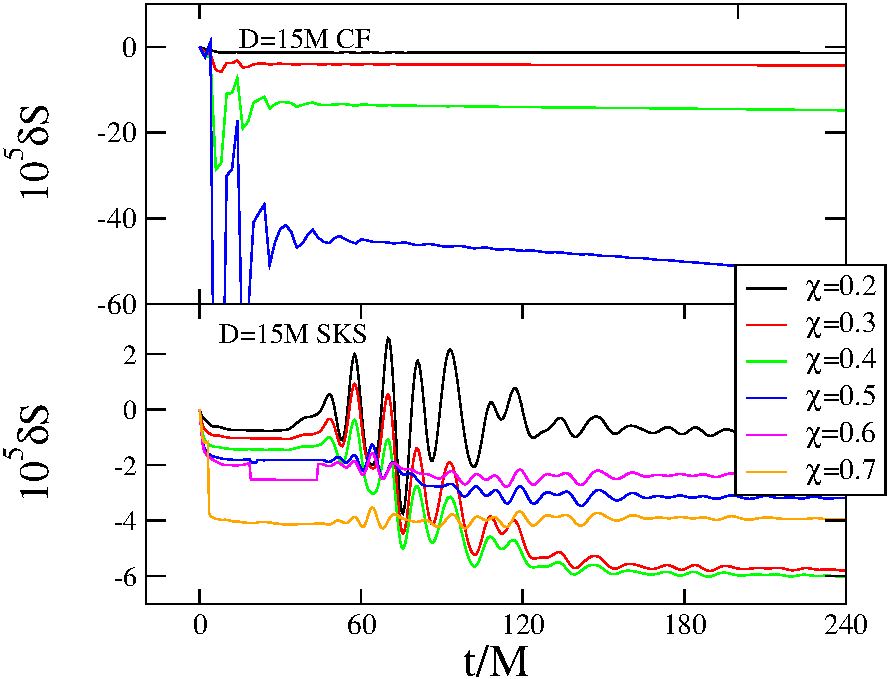
\includegraphics[width=0.95\columnwidth]{chap5/SvsT2}
\caption[$\delta S(t)$ for CF and SKS initial data.]{Fractional change
  in spin relative to $t=0$, $\delta S(t) = S(t)/S(t=0)-1$.  The top
  panel shows CF initial data and the bottom panel SKS data (note the
  different scale).  All simulations shown are at $D=15M$.}
\label{fig:SvsT2}
\end{figure}


\begin{figure}
  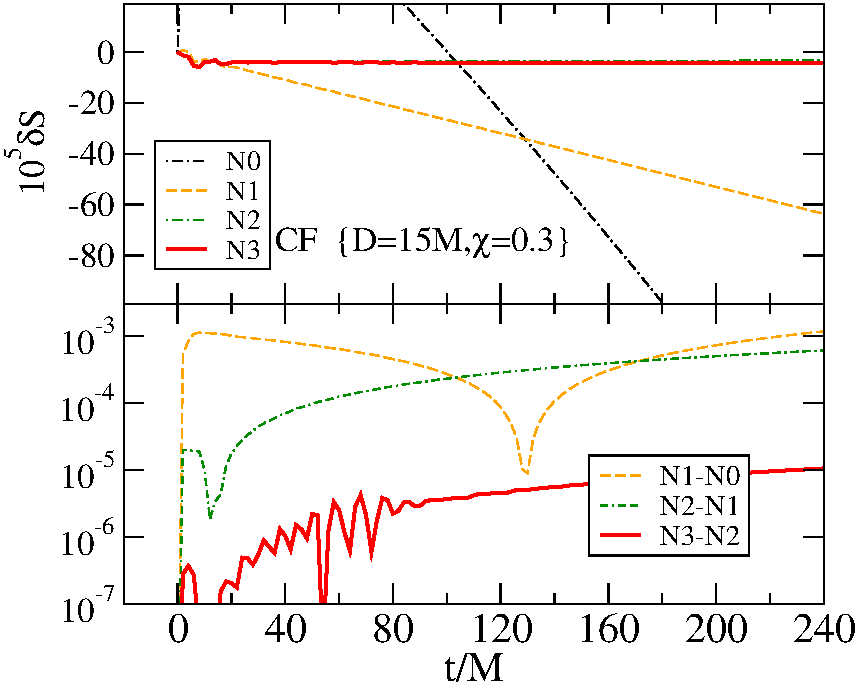
\includegraphics[width=0.95\columnwidth]{chap5/CFSConvergence1}
  \caption[Convergence test of $\delta S(t)$ for CF initial data.]{Convergence test of $\delta S(t)$ for CF initial data in the case
    $\{D=15M,\chi=0.3\}$. The top panel shows $\delta S(t)$ at different
    resolutions and the bottom panel shows the differences between
    consecutive resolutions}
  \label{fig:CFSConvergence1}
\end{figure}

\begin{figure}
  \includegraphics[width=0.95\columnwidth]{chap5/SKSSConvergence1}
  \caption[Convergence test of $\delta S(t)$ for SKS initial data.]{Convergence test of $\delta S(t)$ for SKS initial data in the case
    $\{D=15M,\chi=0.3\}$. The top panel shows $\delta S(t)$ at different
    resolutions and the bottom panel shows the differences between
    consecutive resolutions}
  \label{fig:SKSSConvergence1}
\end{figure}

%\begin{figure}
%  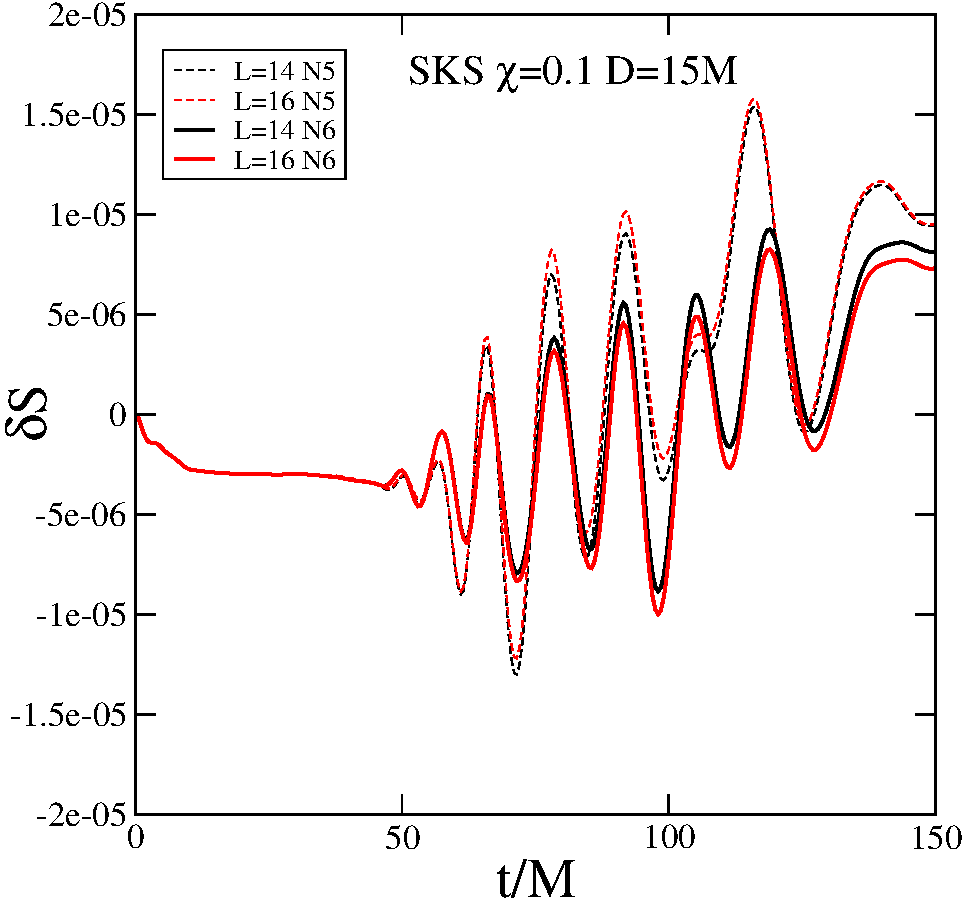
\includegraphics[width=0.95\columnwidth]{chap5/dS_SKS_S1}
%\end{figure}

%\begin{figure}
 % 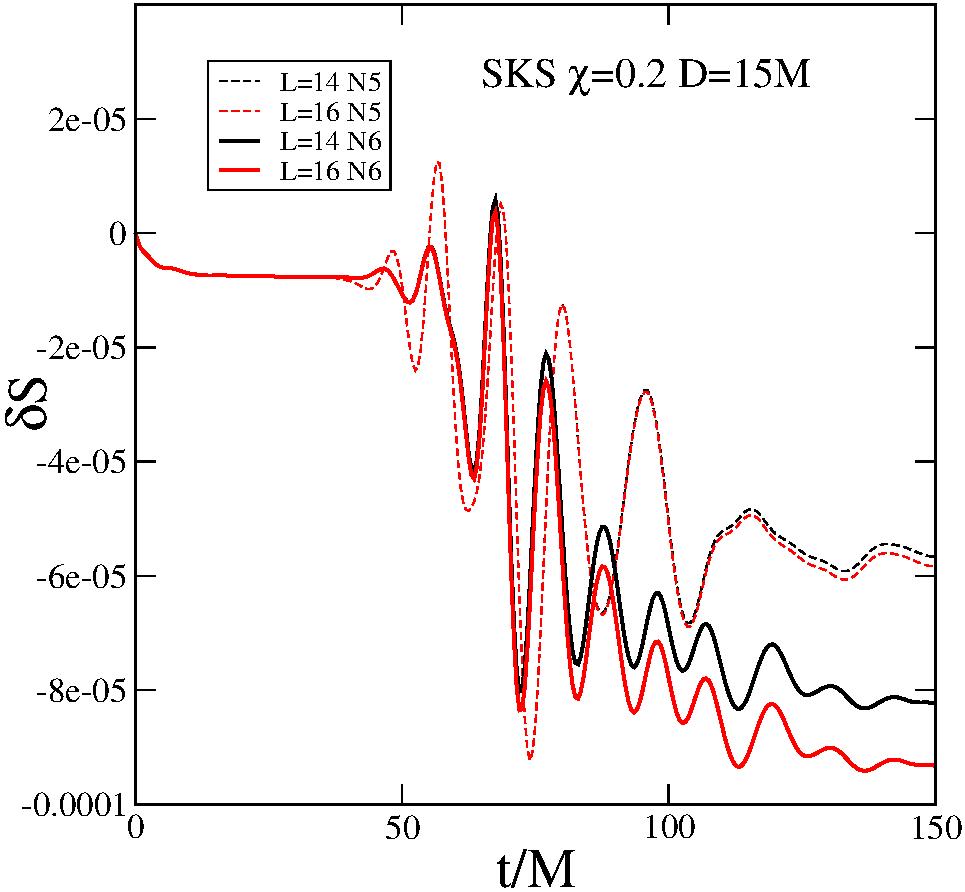
\includegraphics[width=0.95\columnwidth]{chap5/dS_SKS_S2}
%\end{figure}

%\begin{figure}
 % 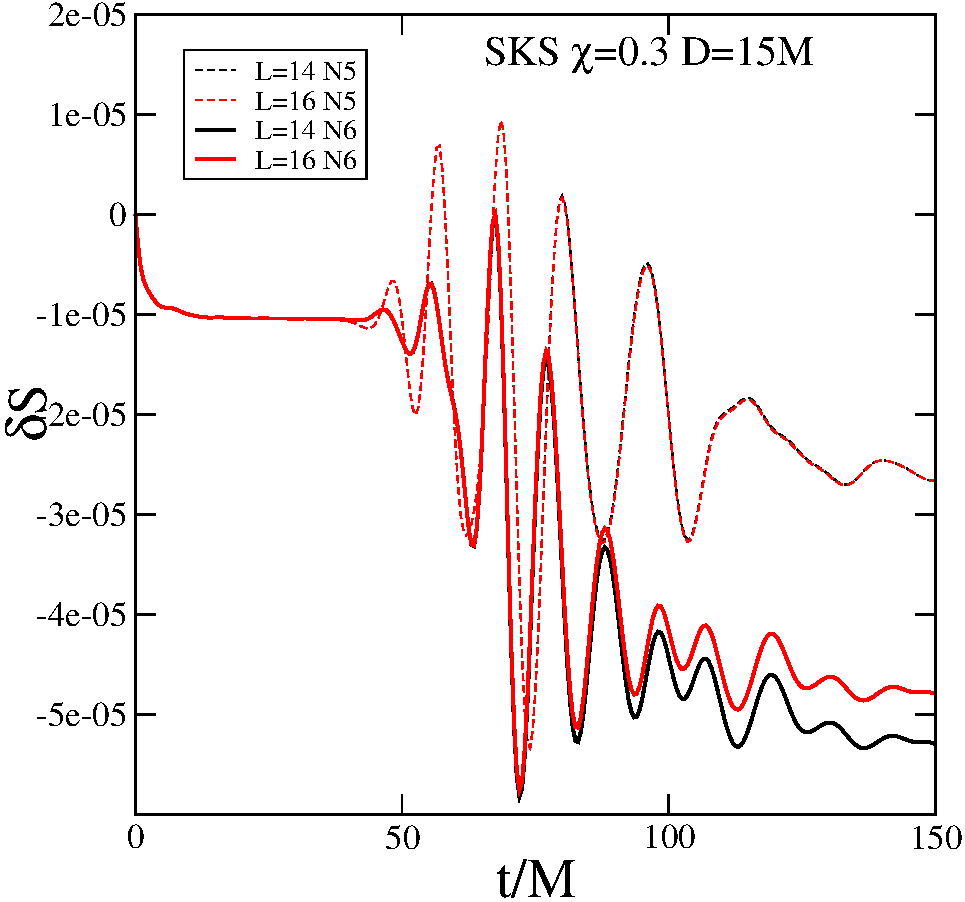
\includegraphics[width=0.95\columnwidth]{chap5/dS_SKS_S3}
%\end{figure}

%\begin{figure}
 % 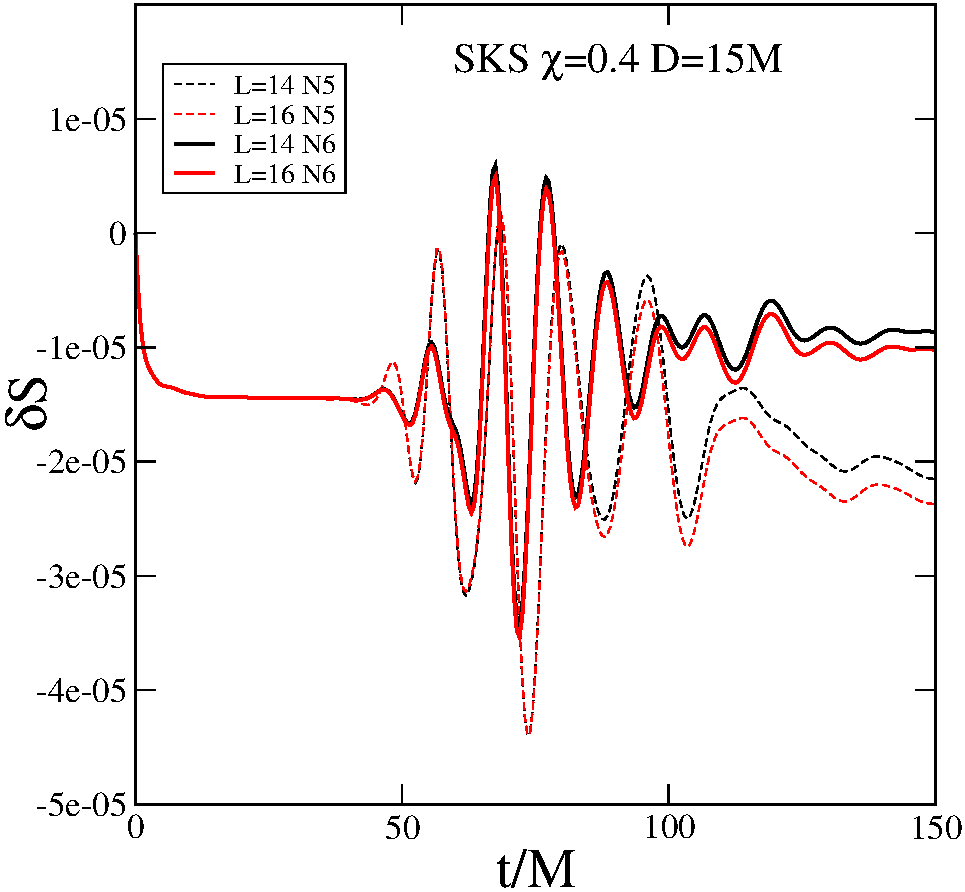
\includegraphics[width=0.95\columnwidth]{chap5/dS_SKS_S4}
%\end{figure}

%\begin{figure}
 % 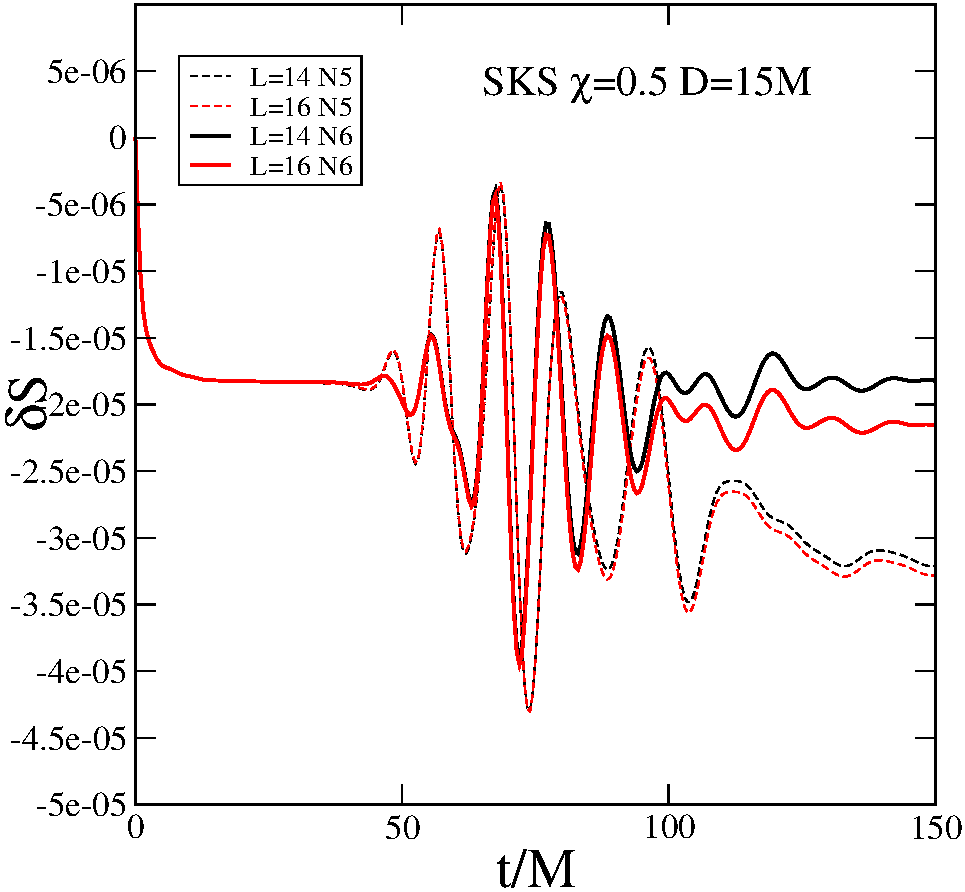
\includegraphics[width=0.95\columnwidth]{chap5/dS_SKS_S5}
%\end{figure}

%\begin{figure}
 % 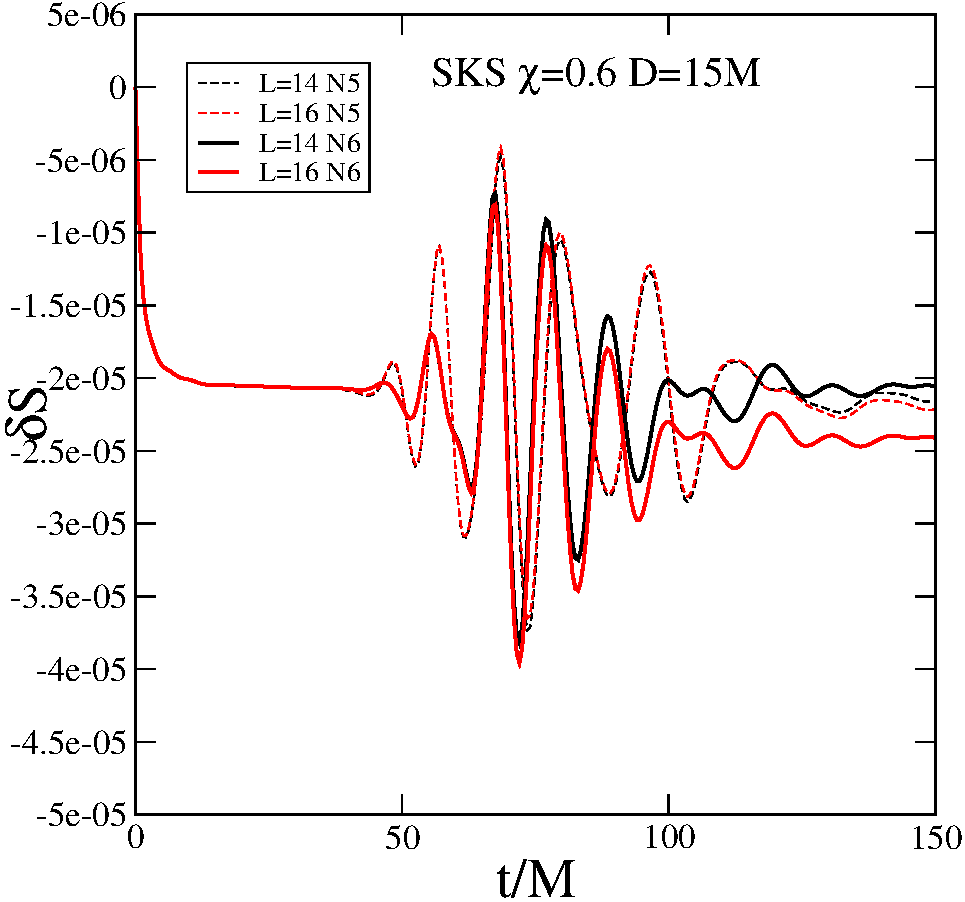
\includegraphics[width=0.95\columnwidth]{chap5/dS_SKS_S6}
%\end{figure}

%\begin{figure}
 % 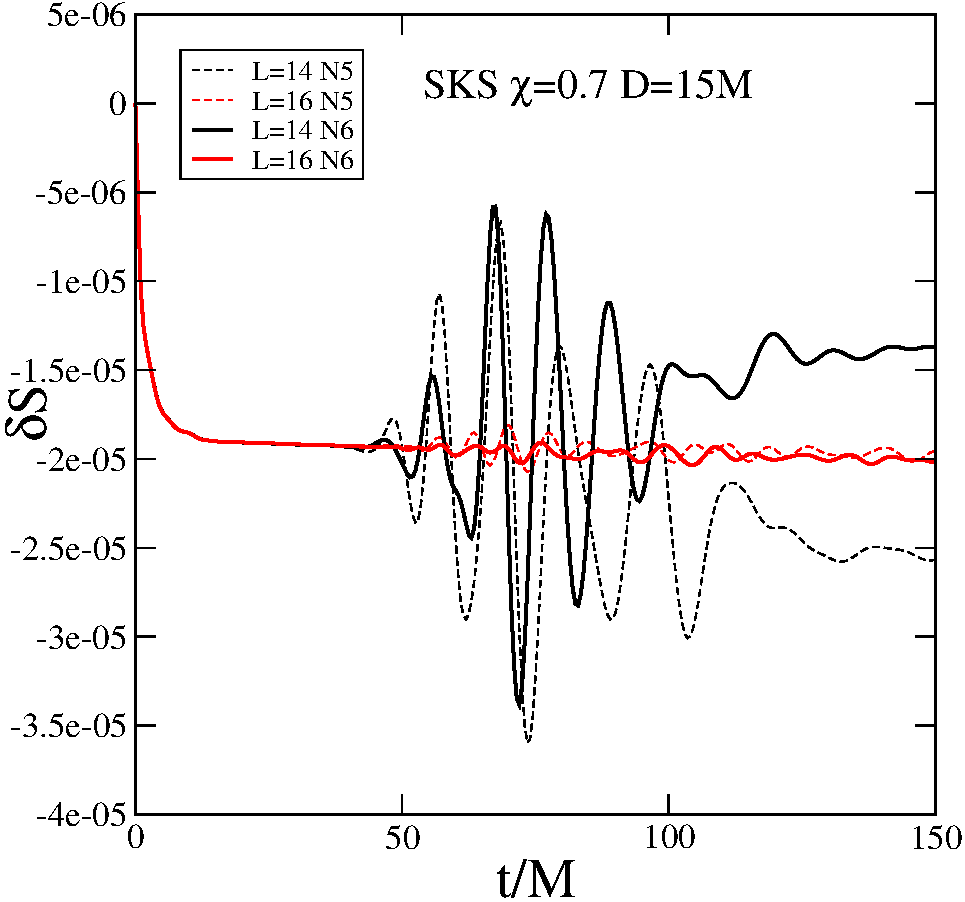
\includegraphics[width=0.95\columnwidth]{chap5/dS_SKS_S7}
%\end{figure}

%\begin{figure}
 % 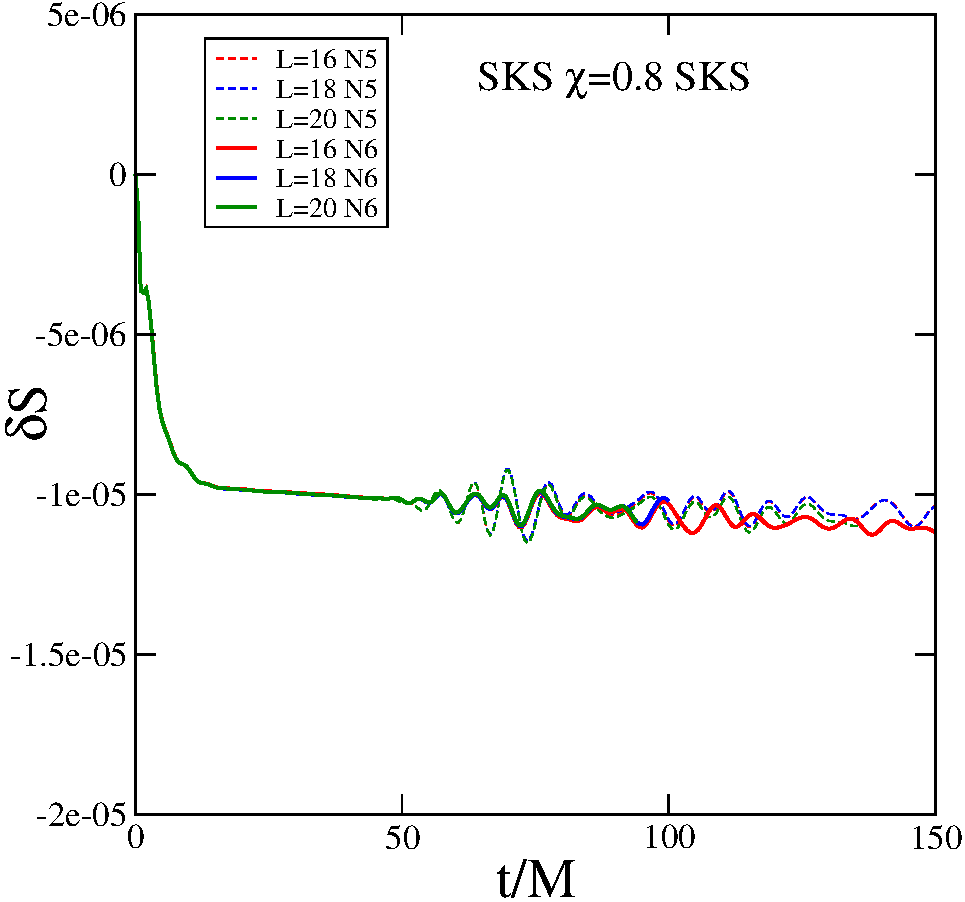
\includegraphics[width=0.95\columnwidth]{chap5/dS_SKS_S8}
%\end{figure}


%\begin{figure}
 % \includegraphics[width=0.99\columnwidth]{SKSSConvergence1}
 % \caption{Same as Fig.~\ref{fig:CFSConvergence1} but for SKS data}
 %\includegraphics[width=0.99\columnwidth]{dsConvTestS8}
 % \caption{Same as above, but $\chi=0.8$}
 % \label{fig:SKSSConvergence1}
%\end{figure}



\section{Results}
\label{sec:Results}




\subsection{Energy in Junk Radiation}

Figure~\ref{fig:EvsS} shows the energy in the pulse of junk radiation,
for all of our runs, as a function of spin. As was expected, the
energy in junk radiation is a decreasing function of initial
separation. We also see that at a given separation and spin, the $E_J$
is always smaller for SKS intiail data than for CF intitial data;
typically by about a factor of 2. Within
the uncertainty of our simulations, $E_J$ has virtually no dependence
on the spins of the black holes. The only exception may be that for
conformally flat data, $E_J$ seems to increase as $\chi\rightarrow
0.5$. This is most visible in the $D=12M$ case. Perhaps the dependence
of $E_J$ on $\chi$ could become important for $\chi > 0.5$ if this
trend continues.

\begin{figure}
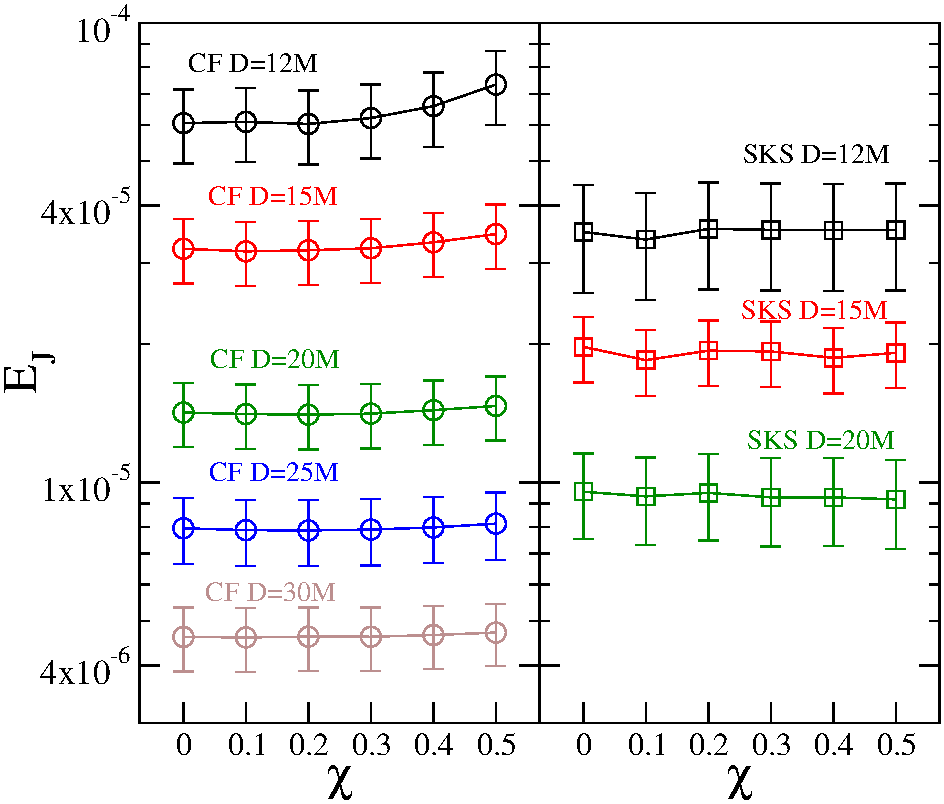
\includegraphics[width=0.95\columnwidth]{chap5/EvsS}
  \caption[$E_J$ as a function of $\chi$.]{Energy in junk radiation as a function of $\chi$ at various
  initial separations, for conformally flat initial data (left panel)
  and SKS initial data (right panel). Within the uncertainty limit,
  there is virtually no dependence of $E_J$ on $\chi$ }
  \label{fig:EvsS}
\end{figure}

Figure~\ref{fig:EvsD} considers the dependence of $E_J$ on the separation $D$ of the black holes. Because there is virtually
no dependence of $E_J$ on $\chi$ (cf. Fig~\ref{fig:EvsS}), we plot only $\chi=0$ in Fig~\ref{fig:EvsD}. $E_J$ vs. $D$ for both CF and SKS data are well approximated by power laws. For
conformally flat data,
\begin{equation}
%E_J^{\rm CF}\sim 0.06225\left(\frac{D}{M}\right)^{-2.7933}.
E_J^{\rm CF}\sim0.062\left(\frac{D}{M}\right)^{-2.79},
\end{equation}
and for SKS data
\begin{equation}
%E_J^{\rm SKS}\sim 0.019576\left(\frac{D}{M}\right)^{-2.5464},
E_J^{\rm SKS}\sim 0.020\left(\frac{D}{M}\right)^{-2.55}.
\end{equation}
Note, however, the latter is a fit to three data points only.

%Figure~\ref{fig:EvsS} shows the energy in junk radiation, $E_J$ as a
%function of a spin. The black curves correspond to conformally flat
%initial data at initial separations of $D=\{12M,15M,20M,25M,30M\}$ and
%the red curves correspond to SKS initial data at initial separations
%of $D=\{12M,15M,20M\}$. Note that this corresponds to all of our data
%from our main runs. It is clear that within the errors of our
%simulations, the junk radiation energy content has virtually no
%dependence on the spin of the black holes. The only exception is that
%for the conformally flat data, $E$ tends to increase as
%$\chi\rightarrow 0.5$. This is most visible in the $D=12M$
%case. Perhaps the dependence of $E_J$ on $\chi$ could become important
%for $\chi>0.5$ if this trend continues.



%Because, as shown in figure~\ref{fig:EvsS}, there is virtually no
%dependence of $E_J$ on $\chi$, in looking at the dependence of $E_J$
%on the initial separation of the black holes, we can look at a fixed
%$\chi$; we choose $\chi=0$. Figure~\ref{fig:EvsD} shows the energy in junk radiation,
%$E_J$ as a function of initial separation, for conformally flat and
%SKS initial data. The dotted lines are the best fit
%power laws to the data. The conformally flat data is a very good fit
%to the power law


\begin{figure}
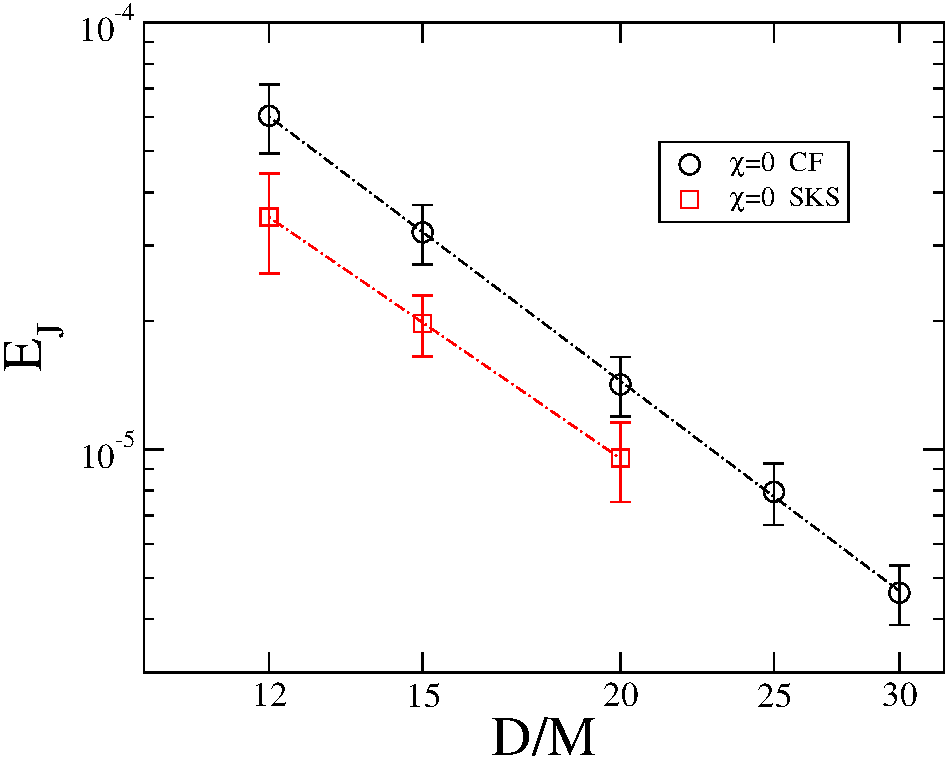
\includegraphics[scale=0.95]{chap5/EvsD}
 \caption[Log-log plot of $E_J$ vs. $D$.]{Log-log plot of the energy in junk radiation as a function
   of initial separation for binaries where $\chi=0$. The black circles and red squares denote conformally flat and SKS initial
   data, respectively. The dotted lines are
   power law fits, with indices of $\sim -2.79$ and $\sim
   -2.55$ respectively.}
 \label{fig:EvsD}
\end{figure}

\subsection{Mass Increase}
\label{subsec:MassIncrease}
We now consider the spin and separation dependence of $\delta M$.
As discussed earlier, we only consider the transient
quantities for CF data, due to the small magnitude of $\delta M$ and $\delta S$ and their non-convergence in SKS data. We
begin by looking at the dependence of $\delta M$ on
separation. In Fig.~\ref{fig:MvsD}, we plot it for curves of
constant $\chi$\footnote{we omit $\chi=0$ because the data is too
  noisy}. 

\begin{figure}[!htbp]
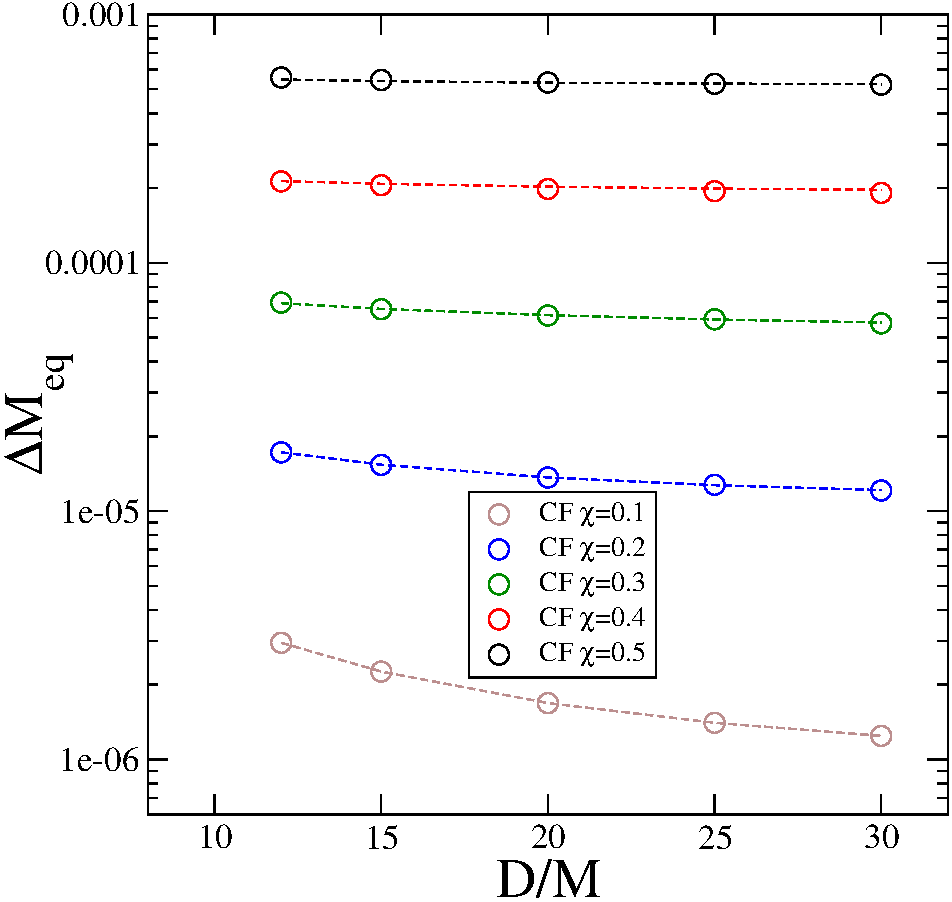
\includegraphics[scale=0.95]{chap5/MvsD2}
\caption[$\delta M$ vs. $D$ for CF initial data.]{$\delta M$ as a function of initial separation for
  CF initial data. The dotted lines are the best fits to a power law
  plus a constant offset.}
\label{fig:MvsD}
\end{figure}

The data are nearly independent of distance at high spin, while there
is a clear dependence at lower spin. In each case, we fit the data to
a power law plus a constant offset. The fits are
\begin{eqnarray*}
\delta M^{\chi = 0.1} &=&
0.00017\left(D/M\right)^{-1.76}+8.19\times 10^{-7}, \\
\delta M^{\chi = 0.2} &=&
0.00021\left(D/M\right)^{-1.36}+1.01\times 10^{-5}, \\
\delta M^{\chi = 0.3} &=&
0.00015\left(D/M\right)^{-0.75}+4.60\times 10^{-5}, \\
\delta M^{\chi = 0.4} &=&
0.00026\left(D/M\right)^{-0.87}+1.83\times 10^{-4}, \\
\delta M^{\chi = 0.5} &=&
0.00047\left(D/M\right)^{-0.99}+5.08\times 10^{-4}. 
\end{eqnarray*}

In Fig.~\ref{fig:MvsS} we show a log-log plot of $\delta M$ on $\chi$ for curves on constant $D$. In each case we compute the best fit power law to the data. These fits are
\begin{eqnarray*}
\delta M^{D=12M} &=& 0.0042\chi^{3.24}, \\
\delta M^{D=15M} &=& 0.0046\chi^{3.39}, \\
\delta M^{D=20M} &=& 0.0052\chi^{3.56}, \\
\delta M^{D=25M} &=& 0.0056\chi^{3.66}, \\
\delta M^{D=30M} &=& 0.0059\chi^{3.74}.
\end{eqnarray*}
We see that the power law exponents are much larger in magnitude than the power law exponents found in the $\delta M$ vs. $D$ fits. This shows that the dependence of $\delta M$ is much stronger on $\chi$ than it is on $D$. If we extrapolate these fits out to $\chi=1$, then $\delta M \sim 0.004-0.006$, which would be an appreciable, although not necessarily limiting, effect.

\begin{figure}[!htbp]
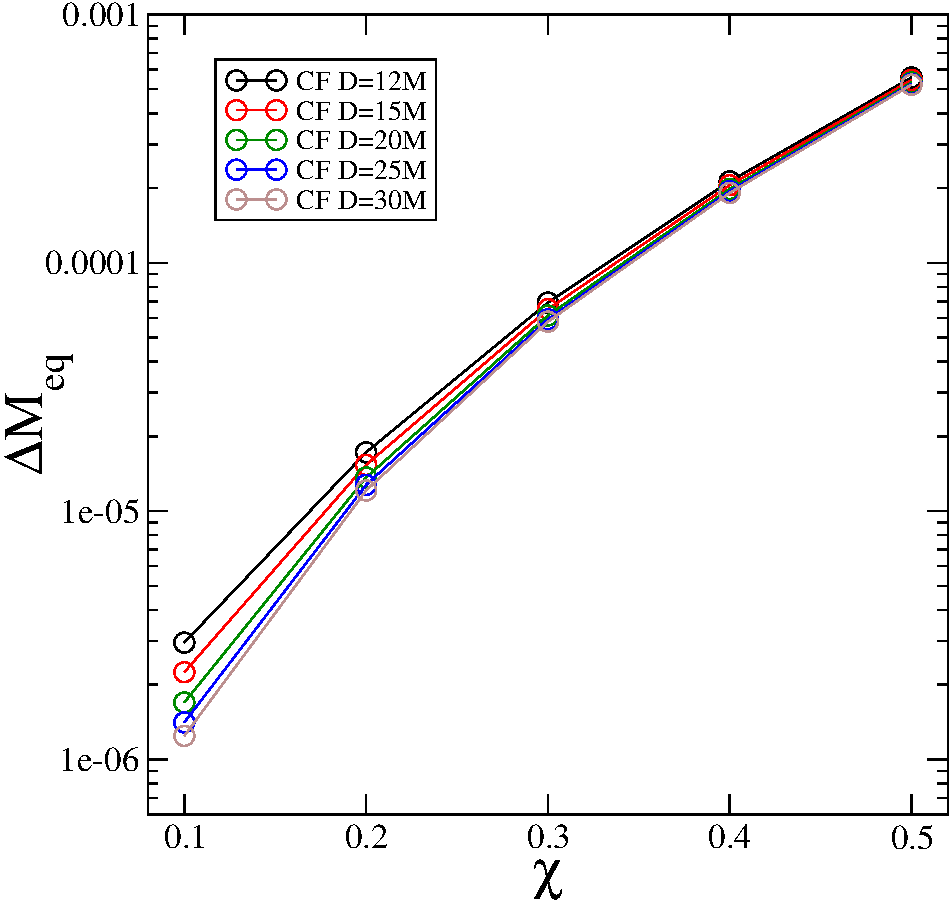
\includegraphics[scale=0.95]{chap5/MvsS2}
 \caption[$\delta M$ as a function of black hole spin $\chi$.]{$\delta M$ as a function of black hole spin $\chi$ for CF
    initial data, evaluated at each different initial separation. The dotted lines are the best fit power laws to the data.}
  \label{fig:MvsS}
\end{figure}


\subsection{Spin Decrease}
\label{subsec:SpinDecrease}
As with the mass increase, we only attempt to calculate $\delta S$ for CF data, as it was found to not be convergent for SKS
data. In Fig.~\ref{fig:SvsD} we plot $\delta S$ vs. $D$ for
curves of constant $\chi$. We omit $\chi=0$ because $\delta
  S$ is not well-defined, and we omit $\chi=0.1$ because the
  data is too noisy. The data are similar to those in
Fig.~\ref{fig:MvsD}, although there seems to be a stronger dependence on initial separation.

\begin{figure}[!htbp]
 \includegraphics[scale=0.95]{chap5/SvsD2}
  \caption[$\delta S$ vs. $D$ for CF initial data.]{$\delta S$ vs. $D$ for CF initial data. The dotted
    curves are the best fit power law plus constant offsets.}
  \label{fig:SvsD}
\end{figure}

In each case, we fit the data to
a power law plus a constant offset. The fits are
\begin{eqnarray*}
\delta S^{\chi = 0.2} &=&
0.00031\left(D/M\right)^{-1.28}+3.70\times 10^{-6}, \\
\delta S^{\chi = 0.3} &=&
0.00034\left(D/M\right)^{-0.84}+6.03\times 10^{-6}, \\
\delta S^{\chi = 0.4} &=&
0.0014\left(D/M\right)^{-1.19}+8.35\times 10^{-5}, \\
\delta S^{\chi = 0.5} &=&
0.0026\left(D/M\right)^{-1.13}+3.45\times 10^{-4}.
\end{eqnarray*}

In figure~\ref{fig:SvsS}, $\delta S$ is plotted as a function
of $\chi$, at different separations. In each case, the data is a good
fit to an exponential; at $D=15M$,
\begin{equation}
\label{eq:spinfit}
\delta S \sim 1.563\times10^{-6}e^{11.546\chi}.
\end{equation}
\begin{figure}[!htbp]
\includegraphics[scale=0.95]{chap5/SvsS2}
\caption[Semi-log plot of $\delta S$ as a function of $\chi$ for CF data.]{Semi-log plot of $\delta S$ as a function of $\chi$ for CF data. The
  dotted lines are the best fit exponentials.}
\label{fig:SvsS}
\end{figure}
Fig. 19 of~\cite{Lovelace2008} found a similar result, noting an exponential relationship between $\Delta \chi$ (defined analogously to $\delta S$ in this chapter) and $\chi(t_{\rm relax})$ for conformally flat initial data. Their relationship is shown from $\chi=0.5$ to $\chi\sim0.93$, however their $\Delta\chi$ matches the $\delta S$ of this chapter in magnitude ($\sim 5\times 10^{-4})$ at $\chi=0.5$, indicating a convergent result between the two works.
If we extrapolate the fit of Eq.~\ref{eq:spinfit} outwards, we find that $\delta S\sim 1$ at
$\chi\sim0.84$. Because this happens before $\chi=1$, this would set a fundamental limit on the highest black
hole spins that can be evolved using conformally flat initial
data. Note that because we fit to $S$ and $\chi$, this limit is
difficult to directly compute. We are only using five data points and extrapolating quite far, so this result must be taken cautiously. However, \cite{Lovelace2008} found a similar maximum spin limit to our extrapolated limit, as they could only evolve CF data
with a maximum spin of $\chi\sim0.93$.



%The dependence of $\Delta S_{eq}$ on the initial separation of the black
%holes is shown in figure ~\ref{fig:SvsD}. We do this for runs where $\chi=0.5$.
%For the CF initial data, we find a good fit a power law with a
%constant offset
%\begin{equation}
%\Delta_S=0.0004139+150.56\left(\frac{D}{M}\right)^{-5.5654}
%\end{equation}
%and we note that for $D>20M$, there is very little dependence on
%$D$. We do not attempt to fit the SKS data, but we note that there is
%a levelling off trend similar to the CF initial data.

%\begin{figure}[!htbp]
% \includegraphics[scale=0.50]{SvsD2}
 % \caption{The dependence of $\Delta S_{eq}$ on the initial separation of
  %  the binaries. The dotted line is the best fit power law plus
   % constant offset to the data, with a power law index of
   % $~-5.57$.\note{Add proper error bars on this fig!}}
  %\label{fig:SvsD}
%\end{figure}

%We begin\note{change wording} by looking at the dependence of $\Delta S_{eq}$ on the spins of
%the black holes. This is shown in figure~\ref{fig:SvsS} for runs where
%$D=15M$, with the black curve as conformally flata initial data, and
%the red curve as SKS initial data. 

%\begin{figure}[!htbp]
%\includegraphics[scale=0.5]{SvsS2}
%\caption{Semi-log plot of the dependence of $\Delta S_{eq}$ on $\chi$. The
%dotted line is the best fit exponential fit to the data}
%\label{fig:SvsS}
%\end{figure}

%In the case of the conformally flat initial data, we find an exponential dependence on
%the spins of the black holes,
%\begin{equation}
%\Delta_S=1.301\times10^{-6}e^{11.672\chi}
%\end{equation}

%\note{change text}For the SKS initial data, we have done runs at an additional three
%points, going up to $\chi=0.8$. Unlike the CF initial data, which has
%a clear exponential dependence on $\chi$, the $\Delta S$ does not seem
%to have any strong dependence on $\chi$, and the oscillations are
%probably due to numerical noise. \note{Need better discussion here}


\section{Conclusion }
\label{sec:JRDiscussion}

We have performed a parameter space study of junk radiation in binary
black hole simulations. We studied the effects of initial separation
and spin magnitude, for spins up to $\chi=0.5$, for both conformally flat and superposed
Kerr-Schild initial data sets. We used three diagnostics to quantify
the amount of junk radiation --- the energy carried away by junk
radiation, the transient mass increase
%\red{better term} 
due to junk radiation and the
transient spin decrease
%\red{better term} 
due to junk radiation.

For the energy present in the junk radiation, $E_J$, we found
very little dependence on the spin of the black holes, but a power law dependence on the initial separations, with exponents of
$\sim -2.79$ for CF initial data and $\sim -2.55$ for SKS initial
data.

We were unable to directly quantify the mass and spin transients for
SKS initial data because of their small magnitudes and a lack of convergence. However, we are
able to say that they are below $\sim 2\times10^{-5}$ and $\sim
4\times10^{-5}$ respectively in the parameter space we study. These
are well below the typical values for CF data, by factors of about 50.

For CF data, for both the mass and spin transients, we see very little
dependence on initial separation. Instead however, we see very strong
dependences on the spin of the black holes, finding an exponential
dependence for $\delta S$ and a steep power law dependence
$\delta M$. Our curves for $\delta S(\chi)$ agree with a previous result found in~\cite{Lovelace2008}. The exponential dependence of 
$\delta S$ on $\chi$ sets a
fundamental limit on the maximum spin of black holes that can be
evolved with conformally flat initial data.
